\chapter{KẾT QUẢ ỨNG DỤNG}
\label{ch:results}

\section{Đặc tả Yêu cầu Phần mềm (SRS)}
\label{sec:srs}

\subsection{Mô tả tổng quan}
\label{subsec:overall_description}

PerFin là ứng dụng mobile quản lý tài chính cá nhân với giao diện hội thoại AI (chatbot) làm trung tâm. Ứng dụng cho phép người dùng ghi chép giao dịch thông qua nhiều phương thức nhập liệu (văn bản, giọng nói, hình ảnh), tự động phân loại và phân tích chi tiêu bằng AI, quản lý ngân sách, theo dõi dòng tiền đa tài khoản, và nhận tư vấn tài chính cá nhân hóa.

\textbf{Đối tượng người dùng mục tiêu:}
\begin{itemize}
    \item Sinh viên, người đi làm trẻ (18--35 tuổi) muốn quản lý tài chính cá nhân nhưng ngại các ứng dụng truyền thống phức tạp.
    \item Người dùng thích giao tiếp bằng ngôn ngữ tự nhiên hơn là điền biểu mẫu.
\end{itemize}

\textbf{Các tác nhân chính (Actors):}

\begin{table}[htbp]
\centering
\begin{tabularx}{\textwidth}{|l|X|}
\hline
\textbf{Actor} & \textbf{Mô tả} \\ \hline
\textbf{User} & Người dùng cuối quản lý tài chính cá nhân \\ \hline
\textbf{AI Engine} & Hệ thống AI xử lý NLP, OCR, Voice-to-Text, phân loại tự động \\ \hline
\textbf{System} & Hệ thống backend tự động (cron jobs, notifications, encryption) \\ \hline
\textbf{Admin/Reviewer} & Quản trị viên duyệt dữ liệu, quản lý danh mục hệ thống \& nhân cách AI \\ \hline
\end{tabularx}
\caption{Các tác nhân trong hệ thống}
\label{tab:actors}
\end{table}

\subsection{Yêu cầu cụ thể}
\label{subsec:specific_requirements}

Hệ thống PerFin được phân tách thành 9 nhóm yêu cầu chính (Requirements), mỗi nhóm đặc tả chi tiết trong tài liệu REQ riêng biệt:

\begin{table}[htbp]
\centering
\begin{tabularx}{\textwidth}{|l|l|X|}
\hline
\textbf{Mã REQ} & \textbf{Tên yêu cầu} & \textbf{Mô tả tóm tắt} \\ \hline
REQ-01 & Nhập liệu đa phương thức bằng AI & Ghi chép giao dịch bằng chat văn bản, giọng nói, hoặc hình ảnh. AI tự động bóc tách dữ liệu. \\ \hline
REQ-02 & Phân loại thông minh & Tự động phân loại giao dịch vào danh mục dựa trên ngữ cảnh, học từ phản hồi người dùng. \\ \hline
REQ-03 & Quản lý Ngân sách & Thiết lập hạn mức chi tiêu, theo dõi tiến độ, cảnh báo chủ động, rollover. \\ \hline
REQ-04 & Phân tích và Báo cáo cá nhân hóa & Biểu đồ trực quan, phát hiện bất thường, tư vấn AI cá nhân hóa. \\ \hline
REQ-05 & Quản lý Tài khoản đa nguồn & Quản lý nhiều ví/tài khoản, chuyển tiền giữa ví, tính tài sản ròng. \\ \hline
REQ-06 & Phân tách Dòng tiền \& Tài sản & Tracking đầu tư, phân biệt Transfer/Investment/Expense, Net Worth, dòng tiền. \\ \hline
REQ-07 & Xuất Dữ liệu \& Sao lưu & Xuất CSV/PDF, sao lưu mã hóa, khôi phục dữ liệu, sao lưu tự động. \\ \hline
REQ-08 & Quản lý Chi phí Cố định \& Nhắc nhở & Chi phí định kỳ, AI nhận diện chu kỳ, nhắc nhở thanh toán, lịch sử thanh toán. \\ \hline
REQ-09 & Nhân cách AI & Phong cách giao tiếp đa dạng, gamification, behavioral psychology. \\ \hline
\end{tabularx}
\caption{Danh sách các yêu cầu hệ thống}
\label{tab:requirements}
\end{table}

\subsection{Yêu cầu chức năng}
\label{subsec:functional_requirements}

\subsubsection{REQ-01: Nhập liệu đa phương thức bằng AI}
\textbf{Tóm tắt:} Cho phép người dùng tạo giao dịch thu/chi mới thông qua giao diện hội thoại bằng văn bản tự nhiên, tin nhắn thoại hoặc hình ảnh. Hệ thống sử dụng AI để đọc hiểu đầu vào tiếng Việt, tiếng Anh hoặc câu pha trộn Việt - Anh; bóc tách tên giao dịch và giá tiền; suy đoán danh mục tương ứng; hỏi lại khi thiếu thông tin.

\textit{Chi tiết đầy đủ: xem phụ lục \ref{sec:appendix_req01}.}

\subsubsection{REQ-02: Phân loại thông minh}
\textbf{Tóm tắt:} Dựa trên ngữ cảnh chat hoặc nội dung hóa đơn, hệ thống tự động phân loại giao dịch vào đúng danh mục. Hỗ trợ danh mục mặc định, danh mục tùy chỉnh, danh mục con, và học từ phản hồi người dùng.

\textit{Chi tiết đầy đủ: xem phụ lục \ref{sec:appendix_req02}.}

\subsubsection{REQ-03: Quản lý Ngân sách}
\textbf{Tóm tắt:} Cho phép thiết lập hạn mức chi tiêu theo danh mục hoặc tổng thể trong kỳ tuần/tháng. Hệ thống tự động theo dõi tiến độ chi tiêu, cảnh báo chủ động tại ngưỡng 70\%, 90\%, 100\%, hỗ trợ rollover ngân sách chưa dùng hết.

\textit{Chi tiết đầy đủ: xem phụ lục \ref{sec:appendix_req03}.}

\subsubsection{REQ-04: Phân tích và Báo cáo cá nhân hóa}
\textbf{Tóm tắt:} Hệ thống tổng hợp dữ liệu giao dịch thành biểu đồ trực quan và đưa ra nhận xét, tư vấn bằng AI dựa trên thói quen chi tiêu thực tế của người dùng. Phát hiện xu hướng bất thường và đưa ra gợi ý cải thiện.

\textit{Chi tiết đầy đủ: xem phụ lục \ref{sec:appendix_req04}.}

\subsubsection{REQ-05: Quản lý Tài khoản đa nguồn}
\textbf{Tóm tắt:} Cho phép tạo và quản lý nhiều ví/tài khoản tài chính (tiền mặt, ngân hàng, ví điện tử, đầu tư). Hỗ trợ chuyển tiền giữa các ví (Transfer), tính tài sản ròng (Net Worth), gán giao dịch vào ví bằng chat.

\textit{Chi tiết đầy đủ: xem phụ lục \ref{sec:appendix_req05}.}

\subsubsection{REQ-06: Phân tách Dòng tiền \& Tài sản}
\textbf{Tóm tắt:} Tracking dòng tiền đầu tư, phân biệt Transfer/Investment/Expense, tính tài sản ròng (Net Worth) chính xác. Theo dõi lãi/lỗ đầu tư cơ bản, báo cáo tổng quan dòng tiền, quản lý dòng tiền bằng chat.

\textit{Chi tiết đầy đủ: xem phụ lục \ref{sec:appendix_req06}.}

\subsubsection{REQ-07: Xuất Dữ liệu \& Sao lưu}
\textbf{Tóm tắt:} Xuất giao dịch ra CSV, xuất báo cáo ra PDF, sao lưu toàn bộ dữ liệu dưới dạng mã hóa, khôi phục dữ liệu, sao lưu tự động định kỳ, yêu cầu xuất/sao lưu qua chat.

\textit{Chi tiết đầy đủ: xem phụ lục \ref{sec:appendix_req07}.}

\subsubsection{REQ-08: Quản lý Chi phí Cố định \& Nhắc nhở}
\textbf{Tóm tắt:} Thiết lập chi phí cố định (tiền nhà, tiền điện, tiền nước...), AI tự động nhận diện chi phí cố định từ lịch sử giao dịch, nhắc nhở chủ động khi đến hạn thanh toán, xác nhận và ghi nhận thanh toán, tạm dừng/kích hoạt lại, theo dõi lịch sử thanh toán.

\textit{Chi tiết đầy đủ: xem phụ lục \ref{sec:appendix_req08}.}

\subsubsection{REQ-09: Nhân cách AI}
\textbf{Tóm tắt:} Chatbot áp dụng các phong cách giao tiếp khác nhau (Chuyên gia tài chính, Bà mẹ nghiêm khắc, Bạn thân, Huấn luyện viên). Mỗi nhân cách ảnh hưởng đến giọng điệu và cách đưa ra lời khuyên nhưng không thay đổi logic xử lý giao dịch.

\textit{Chi tiết đầy đủ: xem phụ lục \ref{sec:appendix_req09}.}

\subsection{Yêu cầu phi chức năng}
\label{subsec:non_functional_requirements}

\begin{table}[htbp]
\centering
\begin{tabularx}{\textwidth}{|l|l|X|}
\hline
\textbf{\#} & \textbf{Yêu cầu} & \textbf{Mô tả} \\ \hline
NFR-01 & Ngôn ngữ & Hệ thống hỗ trợ tiếng Việt, tiếng Anh và câu pha trộn Việt - Anh. \\ \hline
NFR-02 & Hiệu năng & Thời gian phản hồi chat $\le$ 3 giây cho xử lý văn bản, $\le$ 8 giây cho OCR. \\ \hline
NFR-03 & Bảo mật & Mã hóa dữ liệu at-rest (AES-256) và in-transit (TLS 1.2+). JWT cho xác thực. \\ \hline
NFR-04 & Khả dụng & Uptime $\ge$ 99\% cho dịch vụ core (không tính downtime API bên ngoài). \\ \hline
NFR-05 & Khả năng mở rộng & Kiến trúc microservice, có thể scale horizontal từng service. \\ \hline
NFR-06 & Tương thích & Hỗ trợ Android 8.0+ và iOS 14.0+. \\ \hline
NFR-07 & Dữ liệu per-user & Tất cả dữ liệu tài chính là riêng tư, chỉ người sở hữu mới có quyền truy cập. \\ \hline
NFR-08 & Độ chính xác AI & Tỷ lệ phân loại danh mục chính xác $\ge$ 85\% cho danh mục mặc định. \\ \hline
NFR-09 & Sao lưu & Hỗ trợ sao lưu tự động và khôi phục dữ liệu hoàn toàn. \\ \hline
NFR-10 & Xuất dữ liệu & Hỗ trợ xuất CSV và PDF với định dạng chuẩn. \\ \hline
\end{tabularx}
\caption{Các yêu cầu phi chức năng}
\label{tab:nfr}
\end{table}

\vspace{0.5cm}
[TODO --- Bổ sung và chi tiết hóa NFR nếu cần]

\section{Thiết kế Phần mềm}
\label{sec:software_design}

\subsection{Kiến trúc ứng dụng (Application Architecture)}
\label{subsec:app_architecture}

PerFin được xây dựng theo kiến trúc phân tầng (Layered Architecture) kết hợp microservice, bao gồm 5 tầng chính:
\begin{enumerate}
    \item \textbf{Tầng Client (Mobile App):} Giao diện người dùng trên mobile, bao gồm Chat UI, Transaction UI, Report UI, Settings UI.
    \item \textbf{Tầng API Gateway:} Điểm vào duy nhất cho mọi yêu cầu từ client, xử lý rate limiting, routing, kiểm tra xác thực.
    \item \textbf{Tầng Dịch vụ Lõi (Core Services):} Các service nghiệp vụ chính --- Auth, Transaction, Category, Budget, Reminder, Export, Backup, Report, Notification.
    \item \textbf{Tầng Dịch vụ AI:} AI Service điều phối các engine con --- NLP Engine, OCR Engine, Voice-to-Text, Categorization Engine, Personality Engine.
    \item \textbf{Tầng Dữ liệu:} Cơ sở dữ liệu chính (PostgreSQL/MongoDB) và Object Storage (S3) cho ảnh, exports, backups.
\end{enumerate}

\begin{figure}[htbp]
    \centering
    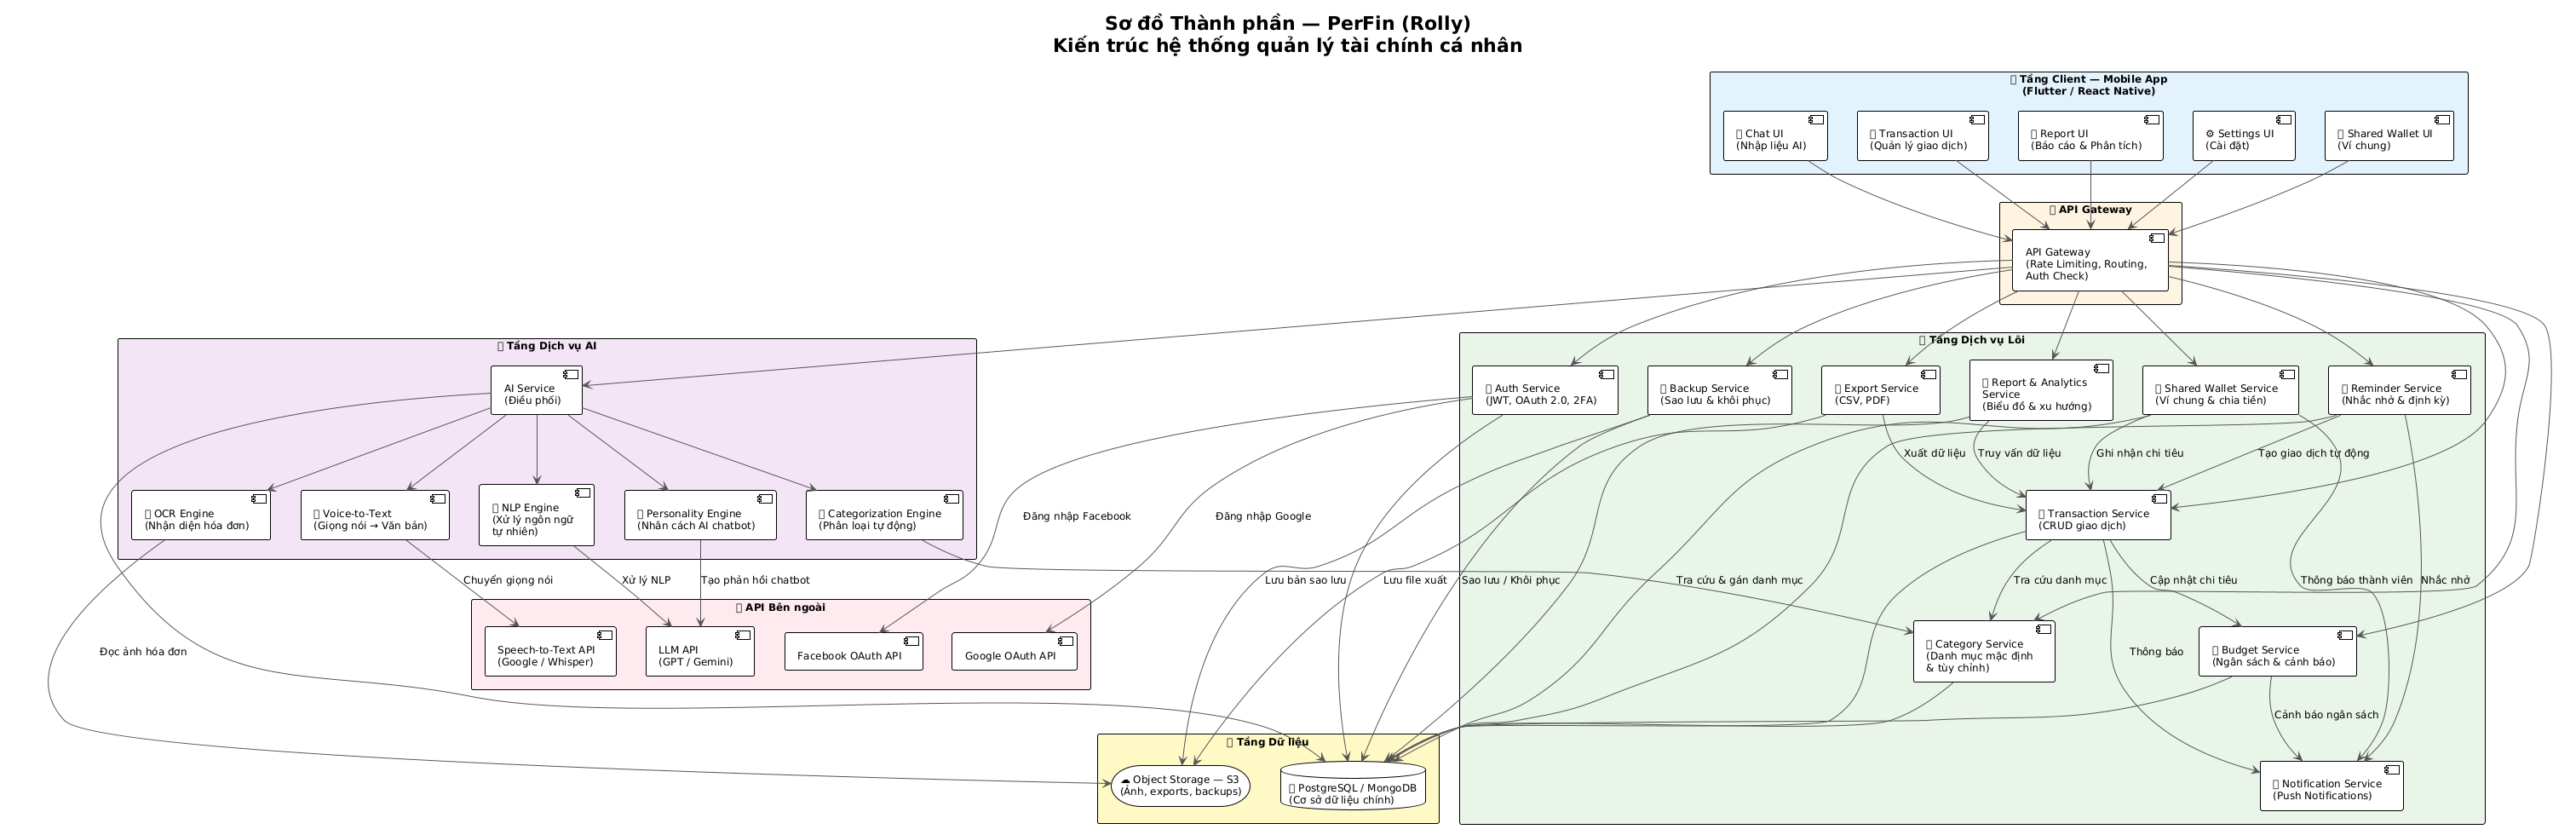
\includegraphics[width=\textwidth]{images/component-diagram.png}
    \caption{Sơ đồ thành phần (Component Diagram)}
    \label{fig:component_diagram}
\end{figure}

[TODO --- Giải thích chi tiết từng tầng sau khi phát triển phần mềm]

\subsection{Thiết kế dữ liệu (Data Design)}
\label{subsec:data_design}

\subsubsection{Sơ đồ lớp (Class Diagram)}
Hệ thống PerFin bao gồm các thực thể (entity) chính:
\begin{itemize}
    \item \textbf{User}: Thông tin người dùng, cài đặt cá nhân.
    \item \textbf{Transaction}: Giao dịch thu/chi/đặc biệt, liên kết với Category và Wallet.
    \item \textbf{Category}: Danh mục giao dịch (mặc định và tùy chỉnh), hỗ trợ cấu trúc cha-con.
    \item \textbf{Wallet}: Ví/tài khoản tài chính (tiền mặt, ngân hàng, ví điện tử, đầu tư).
    \item \textbf{Budget}: Ngân sách theo danh mục hoặc tổng thể, với kỳ tuần/tháng.
    \item \textbf{Reminder}: Nhắc nhở giao dịch và chi phí cố định.
    \item \textbf{AIPersonality}: Nhân cách AI chatbot.
    \item \textbf{ChatMessage}: Lưu trữ lịch sử hội thoại.
\end{itemize}

\begin{figure}[htbp]
    \centering
    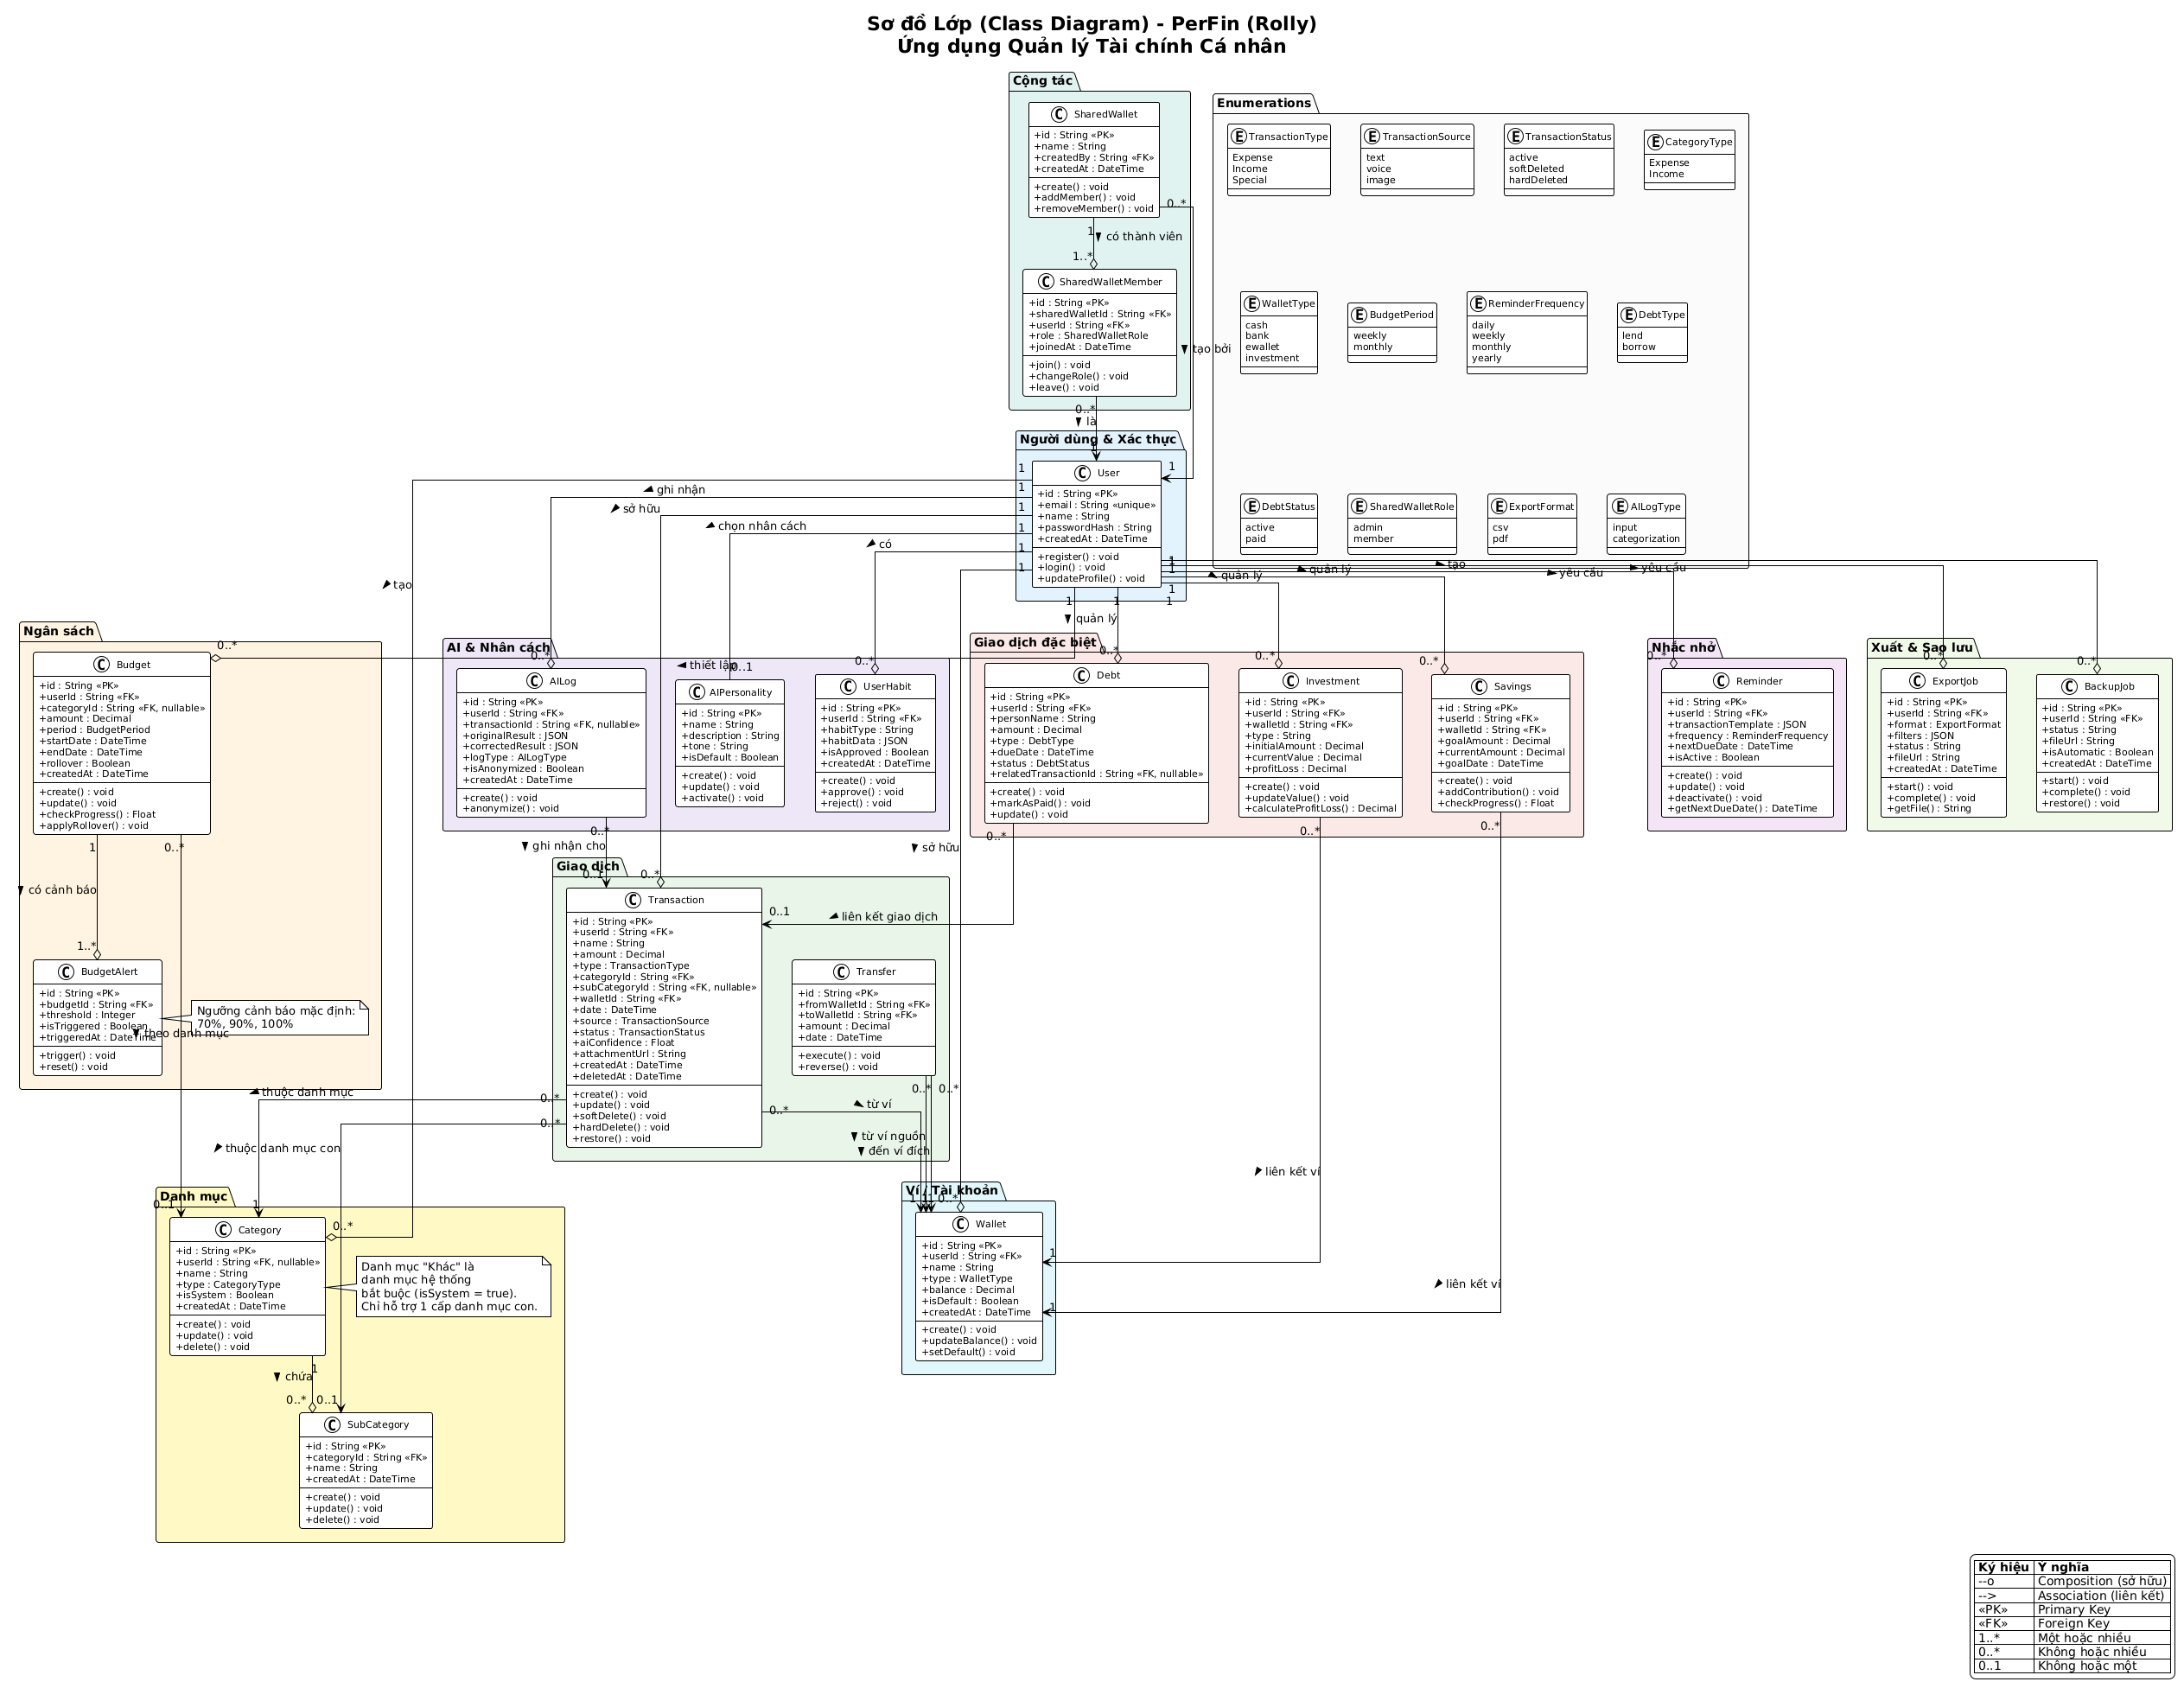
\includegraphics[width=\textwidth]{images/class-diagram.png}
    \caption{Sơ đồ lớp (Class Diagram)}
    \label{fig:class_diagram}
\end{figure}

[TODO --- Giải thích các quan hệ giữa các thực thể sau khi hoàn thiện cơ sở dữ liệu]

\subsubsection{Sơ đồ quan hệ thực thể (ERD)}

\begin{figure}[htbp]
    \centering
    %\includegraphics[width=0.8\textwidth]{diagrams/erd-diagram.png}
    \fbox{\parbox{0.8\textwidth}{\centering\vspace{1.5cm} Sơ đồ thực thể quan hệ (ERD) \\ (Vẽ ERD từ Class Diagram, thêm các trường dữ liệu và kiểu dữ liệu)\vspace{1.5cm}}}
    \caption{Sơ đồ quan hệ thực thể (ERD)}
    \label{fig:erd_diagram}
\end{figure}

[TODO --- Tạo ERD từ Class Diagram, bổ sung các trường dữ liệu, kiểu dữ liệu, khóa chính, khóa ngoại]

\subsection{Thiết kế chi tiết (Detailed Design)}
\label{subsec:detailed_design}

\subsubsection{Sơ đồ Use Case tổng quan}
Sơ đồ Use Case mô tả tổng quan các tác nhân và chức năng chính của hệ thống PerFin, được tổ chức theo 9 nhóm yêu cầu (REQ-01 đến REQ-09).

Do sơ đồ Use Case tổng quan chứa số lượng lớn các chức năng (từ REQ-01 đến REQ-10) nên rất lớn và khó quan sát đầy đủ trên một trang tài liệu. Vì vậy, sơ đồ được chia nhỏ thành 1 sơ đồ tổng quan mức cao (hệ thống) và 3 sơ đồ chi tiết theo các nhóm chức năng:

\begin{figure}[htbp]
    \centering
    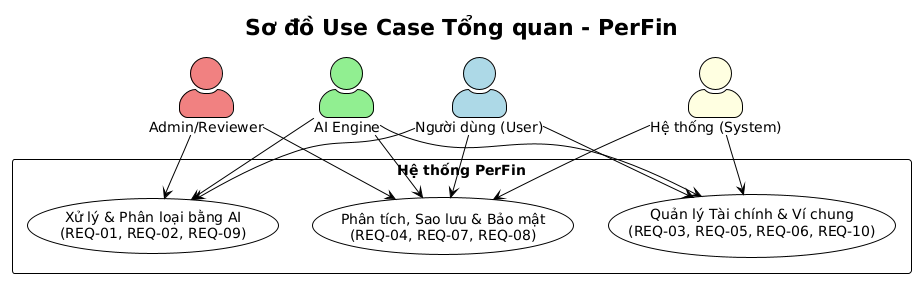
\includegraphics[width=0.9\textwidth]{images/use-case-diagram.png}
    \caption{Sơ đồ Use Case tổng quan mức cao (Overview)}
    \label{fig:use_case_overview}
\end{figure}

\begin{figure}[htbp]
    \centering
    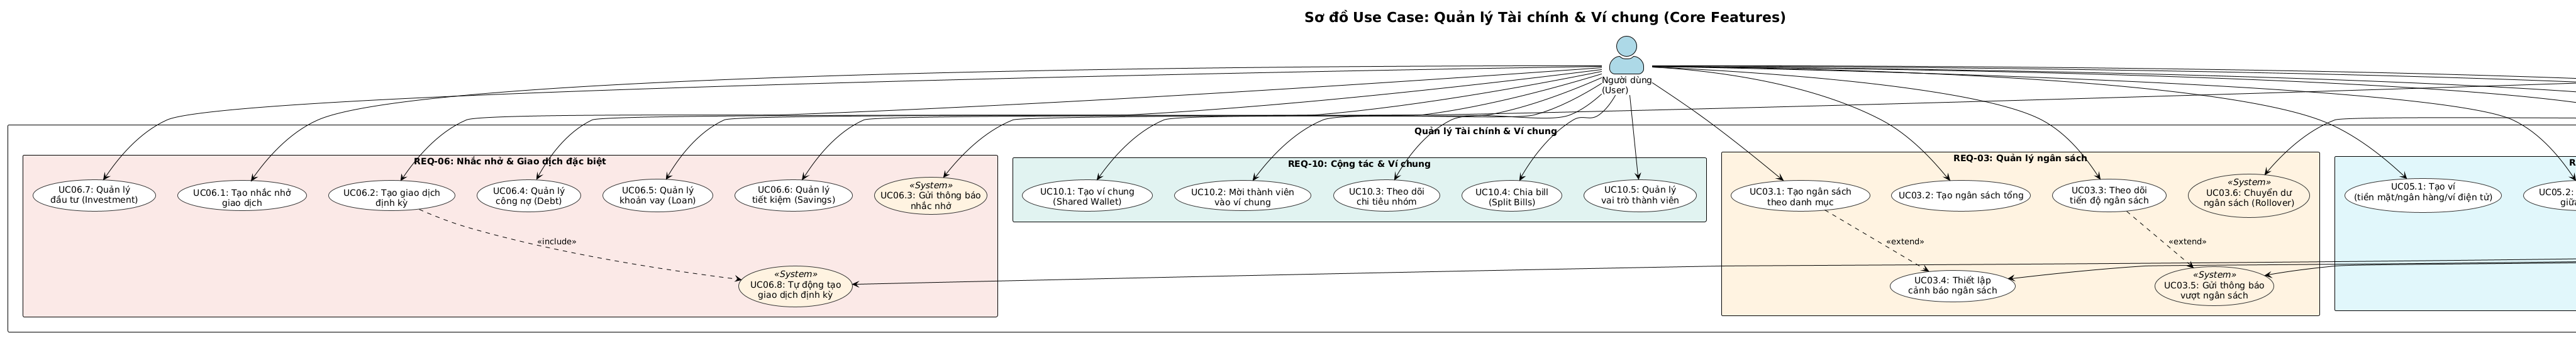
\includegraphics[width=0.95\textwidth]{images/use-case-core.png}
    \caption{Sơ đồ Use Case phân hệ Quản lý Tài chính \& Ví chung (Core Features)}
    \label{fig:use_case_core}
\end{figure}

\begin{figure}[htbp]
    \centering
    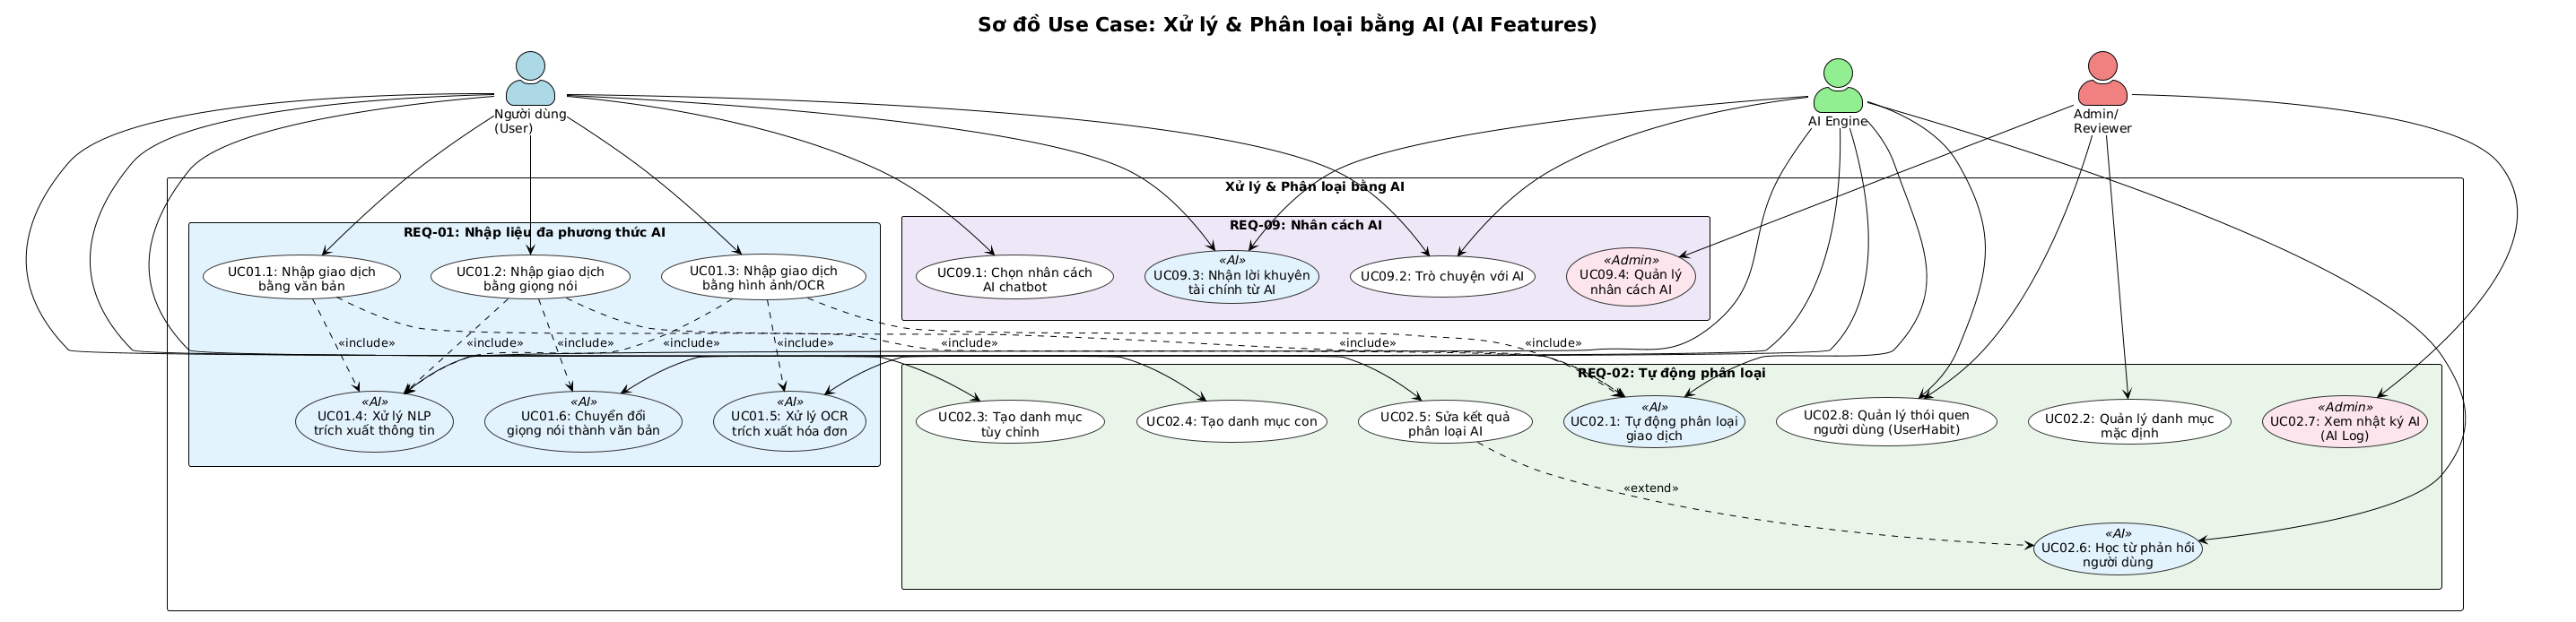
\includegraphics[width=0.95\textwidth]{images/use-case-ai.png}
    \caption{Sơ đồ Use Case phân hệ Xử lý \& Phân loại bằng AI (AI Features)}
    \label{fig:use_case_ai}
\end{figure}

\begin{figure}[htbp]
    \centering
    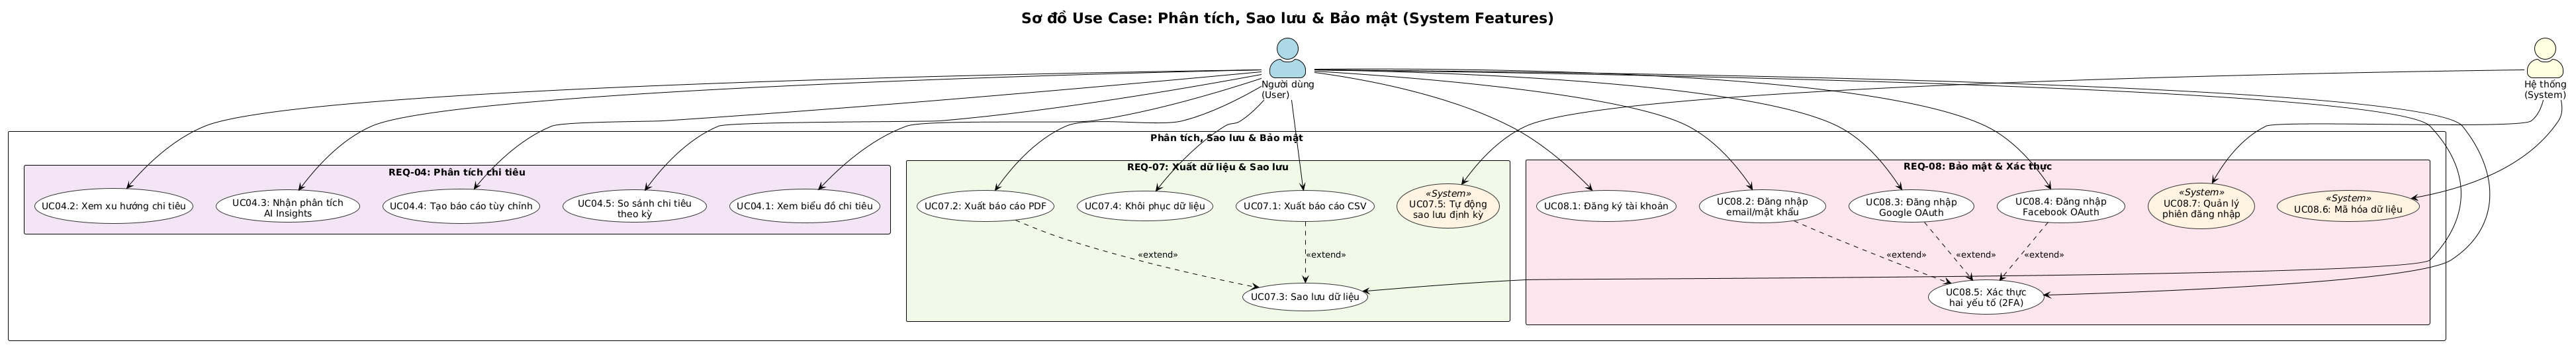
\includegraphics[width=0.95\textwidth]{images/use-case-system.png}
    \caption{Sơ đồ Use Case phân hệ Phân tích, Sao lưu \& Bảo mật (System Features)}
    \label{fig:use_case_system}
\end{figure}

[TODO --- Giải thích chi tiết use case]

\subsubsection{Sơ đồ tuần tự (Sequence Diagrams)}
Các sơ đồ tuần tự mô tả luồng tương tác giữa các tác nhân và hệ thống cho các use case quan trọng.

Các sơ đồ tuần tự chi tiết hóa luồng tương tác giữa các tác nhân (Người dùng, AI Engine, Hệ thống) và các dịch vụ bên trong hệ thống đối với từng nghiệp vụ cụ thể:

\begin{figure}[htbp]
    \centering
    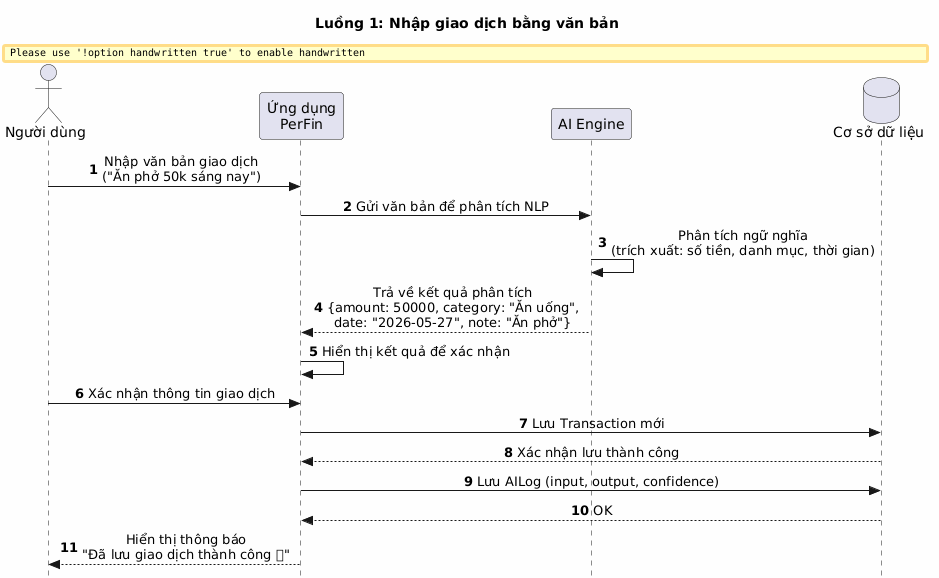
\includegraphics[width=0.9\textwidth]{images/sequence-nhập-giao-dịch-bằng-văn-bản.png}
    \caption{Sơ đồ tuần tự: Nhập giao dịch bằng văn bản}
    \label{fig:seq_text_input}
\end{figure}

\begin{figure}[htbp]
    \centering
    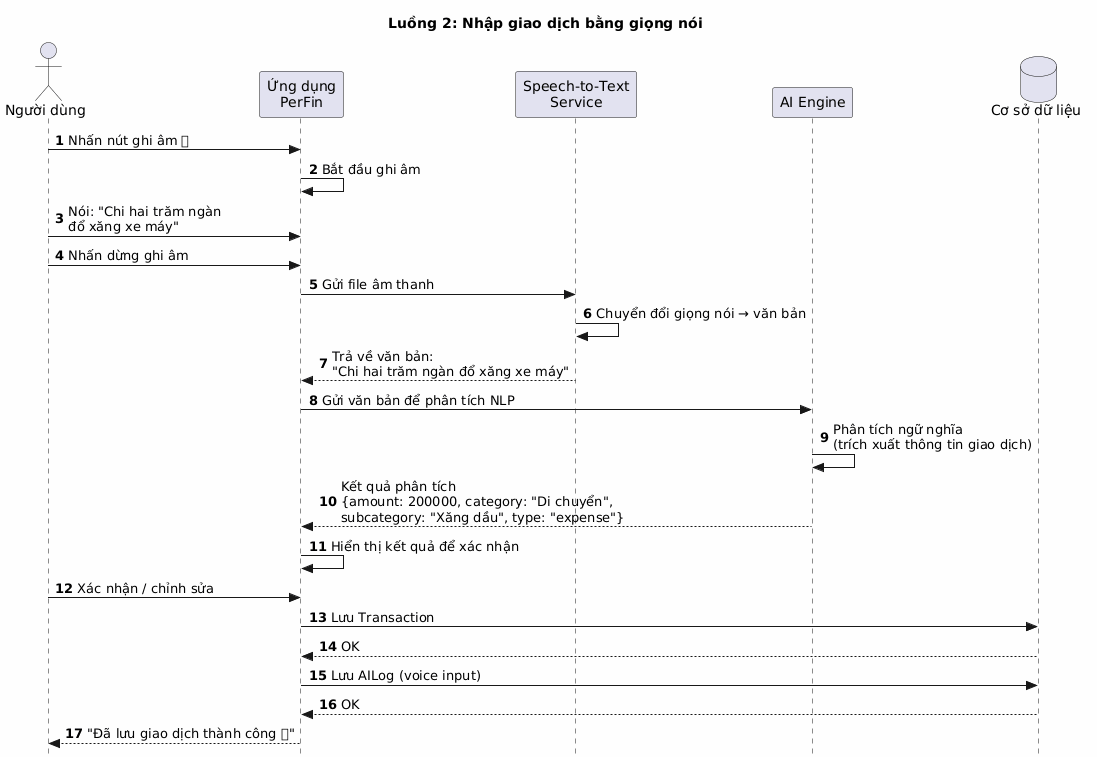
\includegraphics[width=0.9\textwidth]{images/sequence-nhập-giao-dịch-bằng-giọng-nói.png}
    \caption{Sơ đồ tuần tự: Nhập giao dịch bằng giọng nói}
    \label{fig:seq_voice_input}
\end{figure}

\begin{figure}[htbp]
    \centering
    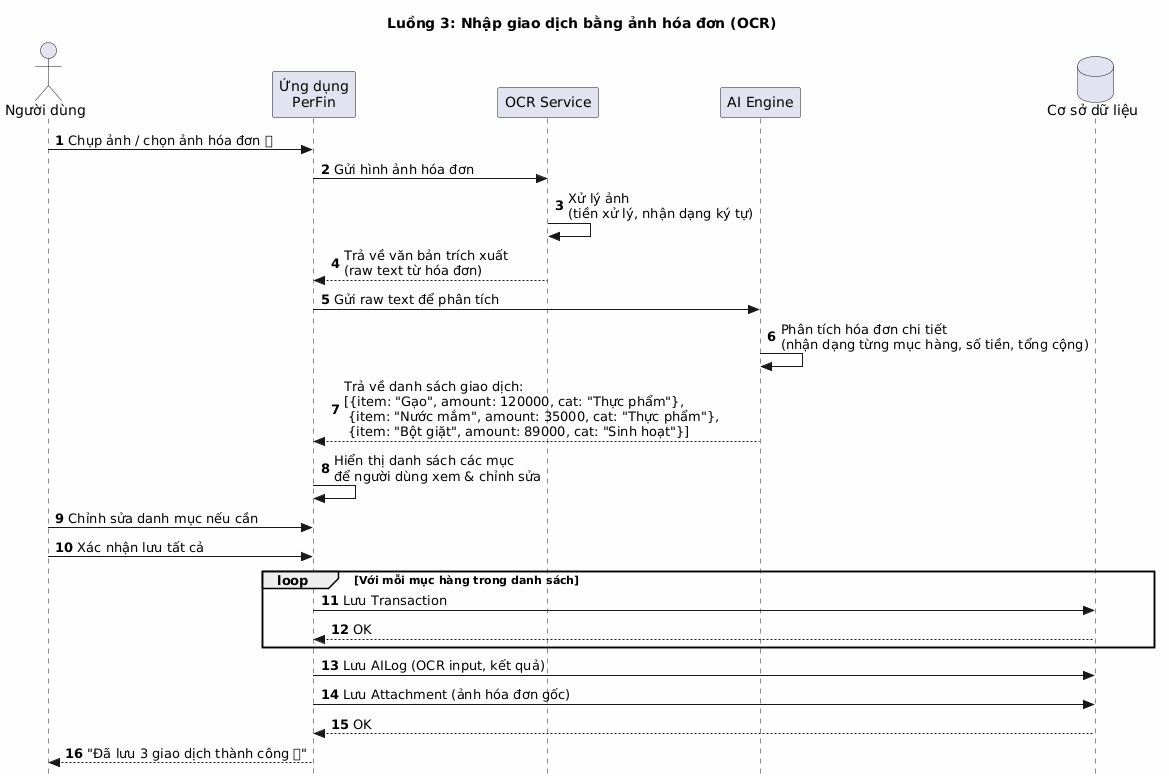
\includegraphics[width=0.9\textwidth]{images/sequence-nhập-giao-dịch-bằng-ảnh-hóa-đơn-ocr.png}
    \caption{Sơ đồ tuần tự: Nhập giao dịch bằng ảnh hóa đơn (OCR)}
    \label{fig:seq_ocr_input}
\end{figure}

\begin{figure}[htbp]
    \centering
    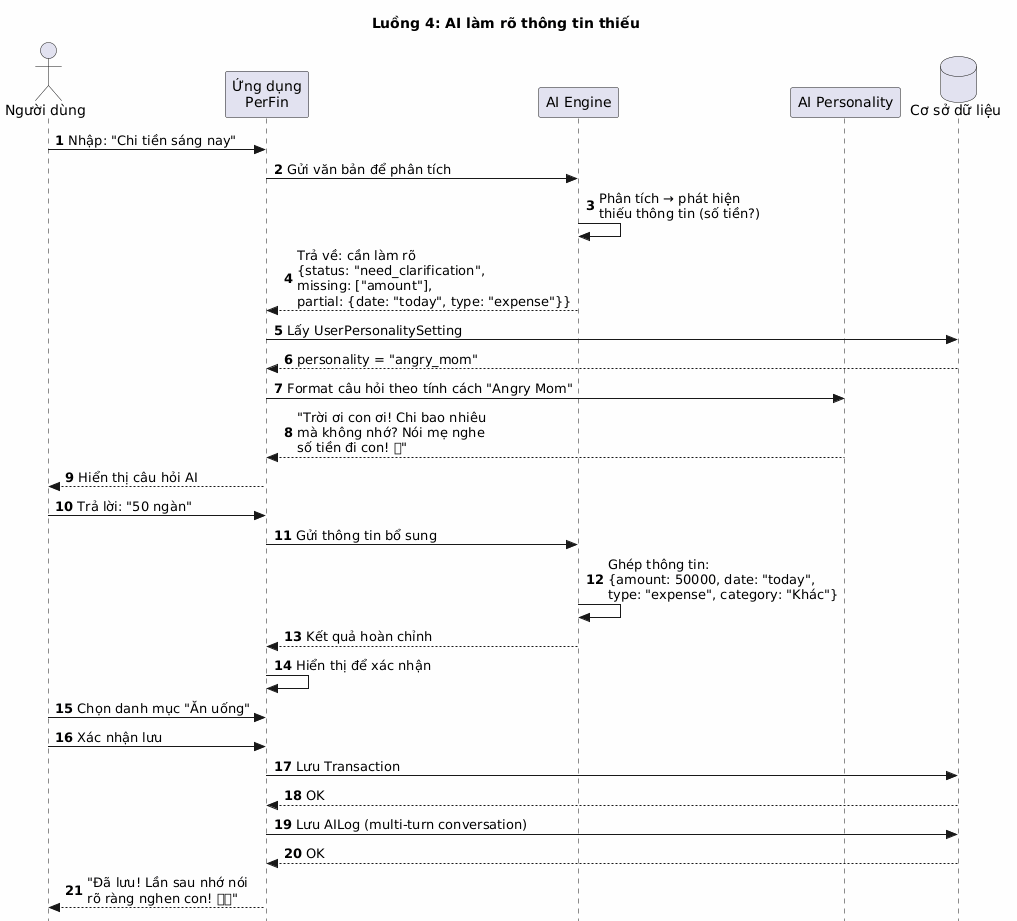
\includegraphics[width=0.9\textwidth]{images/sequence-ai-làm-rõ-thông-tin-thiếu.png}
    \caption{Sơ đồ tuần tự: AI làm rõ thông tin thiếu}
    \label{fig:seq_ai_clarify}
\end{figure}

\begin{figure}[htbp]
    \centering
    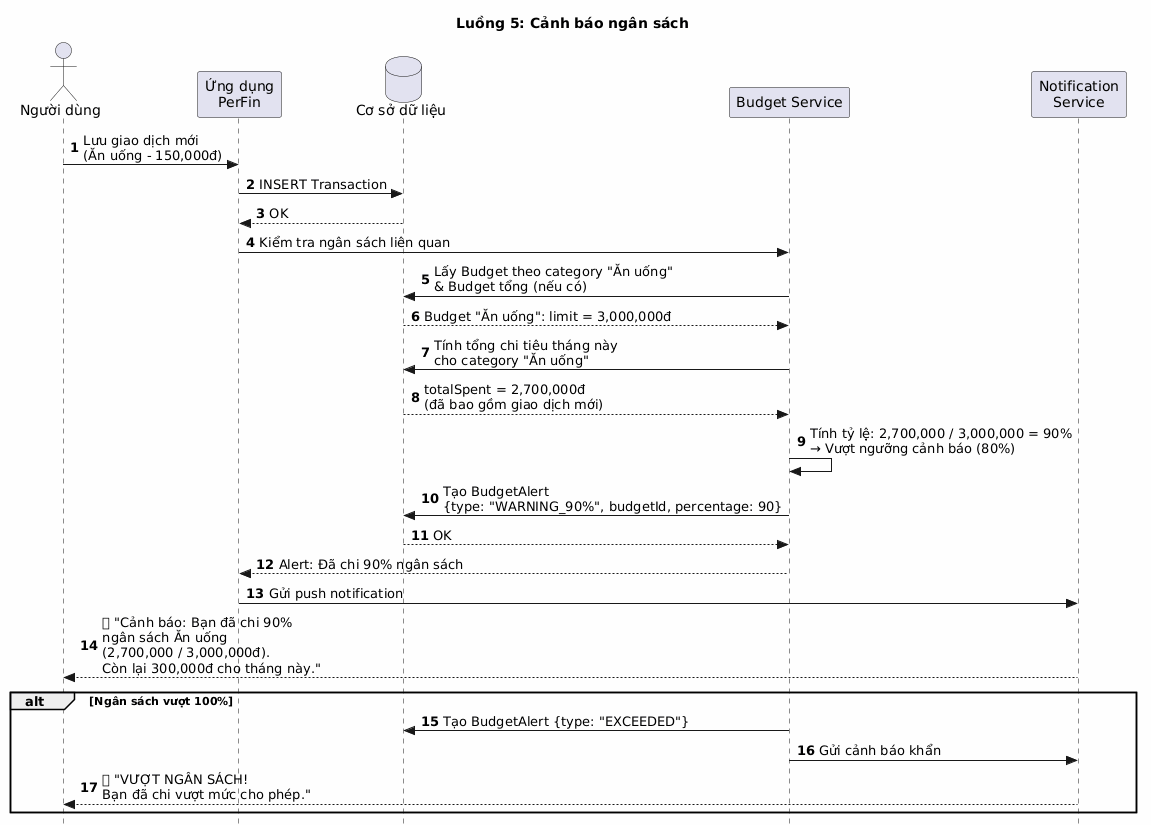
\includegraphics[width=0.9\textwidth]{images/sequence-cảnh-báo-ngân-sách.png}
    \caption{Sơ đồ tuần tự: Cảnh báo ngân sách}
    \label{fig:seq_budget_alert}
\end{figure}

\begin{figure}[htbp]
    \centering
    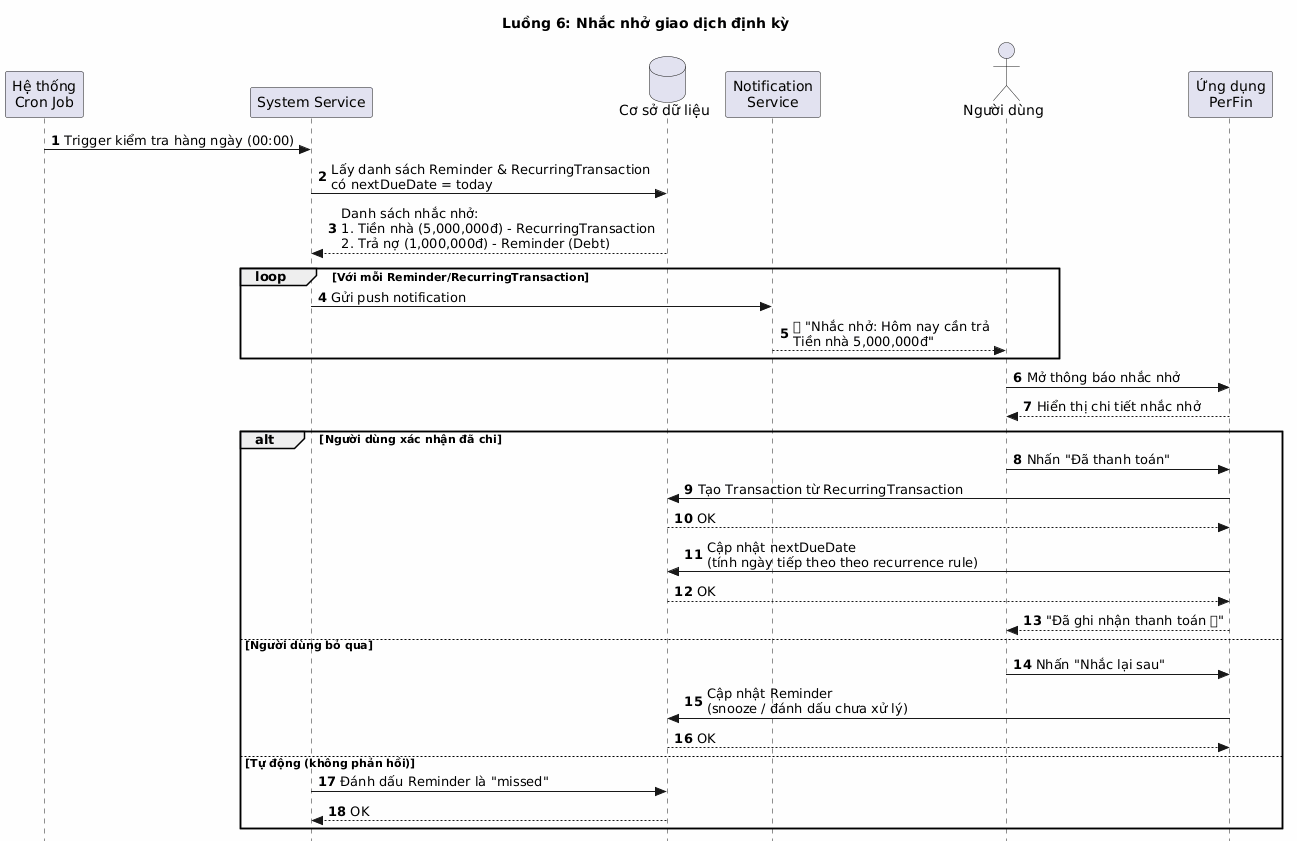
\includegraphics[width=0.9\textwidth]{images/sequence-nhắc-nhở-giao-dịch-định-kỳ.png}
    \caption{Sơ đồ tuần tự: Nhắc nhở giao dịch định kỳ}
    \label{fig:seq_recurring_reminder}
\end{figure}

\begin{figure}[htbp]
    \centering
    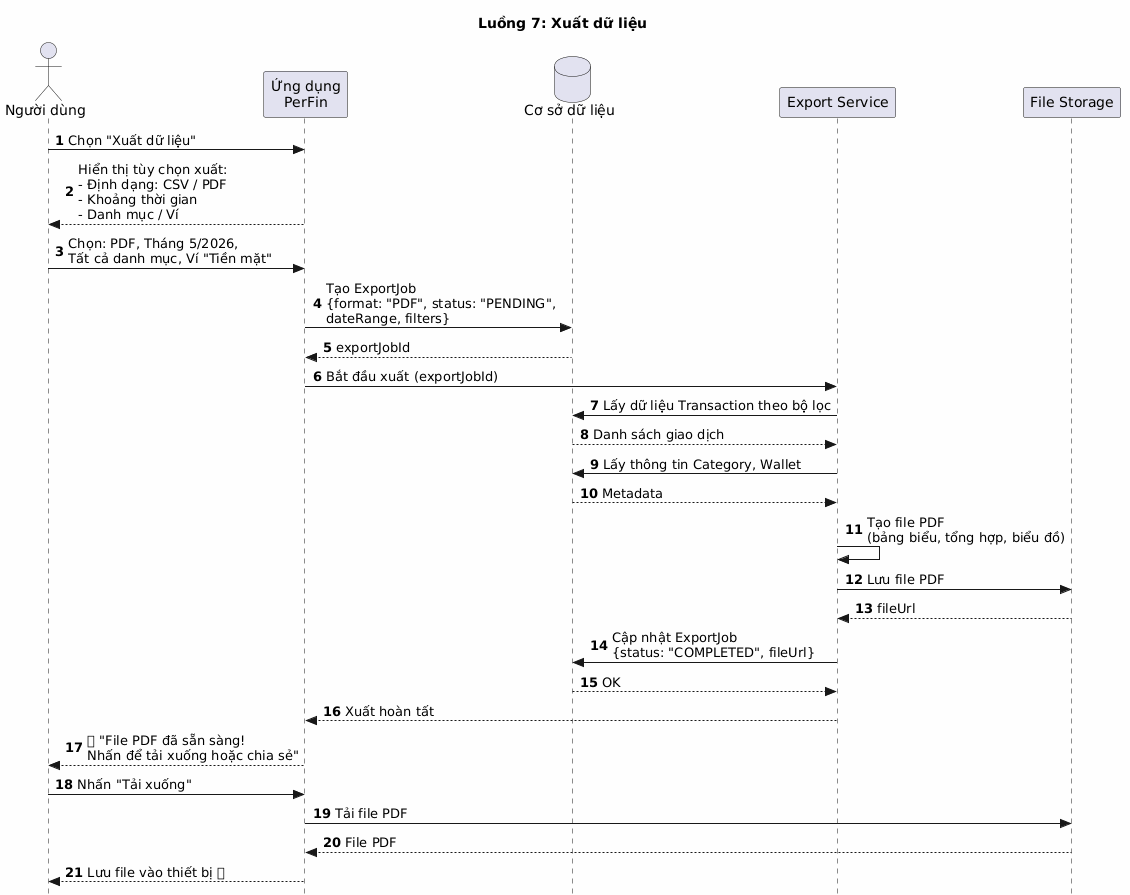
\includegraphics[width=0.9\textwidth]{images/sequence-xuất-dữ-liệu.png}
    \caption{Sơ đồ tuần tự: Xuất dữ liệu}
    \label{fig:seq_export_data}
\end{figure}

\begin{figure}[htbp]
    \centering
    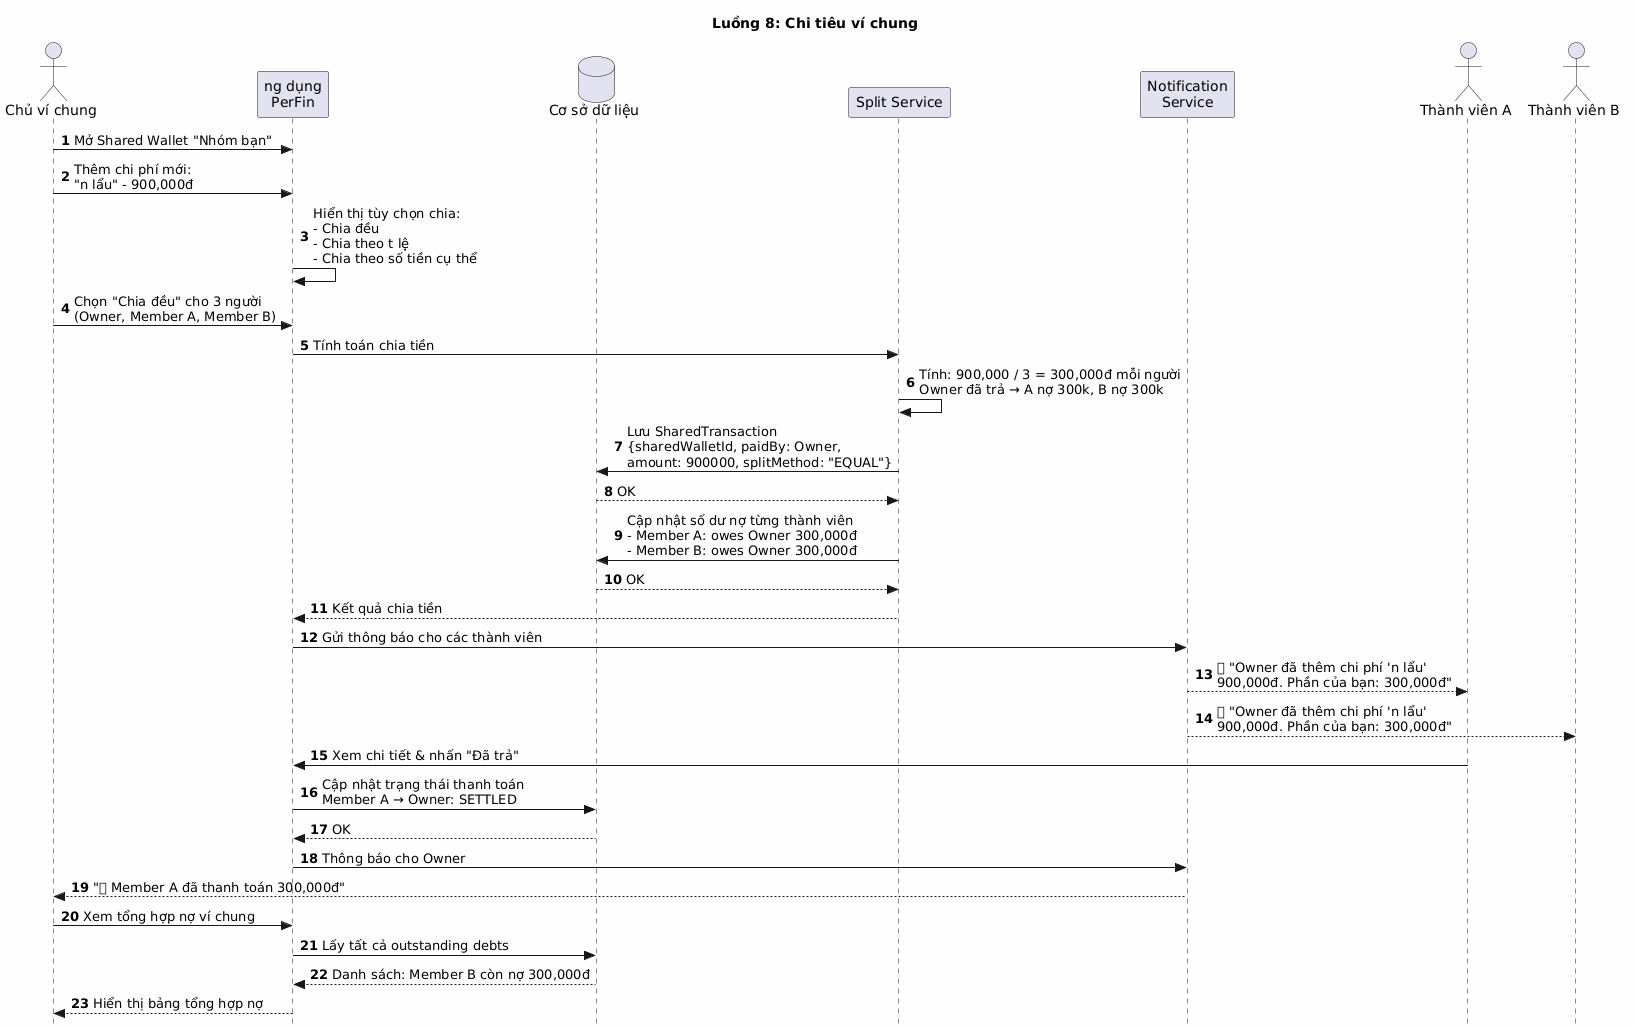
\includegraphics[width=0.9\textwidth]{images/sequence-chi-tiêu-ví-chung.png}
    \caption{Sơ đồ tuần tự: Chi tiêu ví chung}
    \label{fig:seq_shared_wallet}
\end{figure}

[TODO --- Giải thích các luồng tương tác chính]

\subsubsection{Sơ đồ hoạt động (Activity Diagrams)}
Các sơ đồ hoạt động mô tả chi tiết quy trình xử lý cho các luồng nghiệp vụ phức tạp.

Các sơ đồ hoạt động mô tả chi tiết quy trình xử lý và logic nghiệp vụ bên trong hệ thống cho các tính năng phức tạp:

\begin{figure}[htbp]
    \centering
    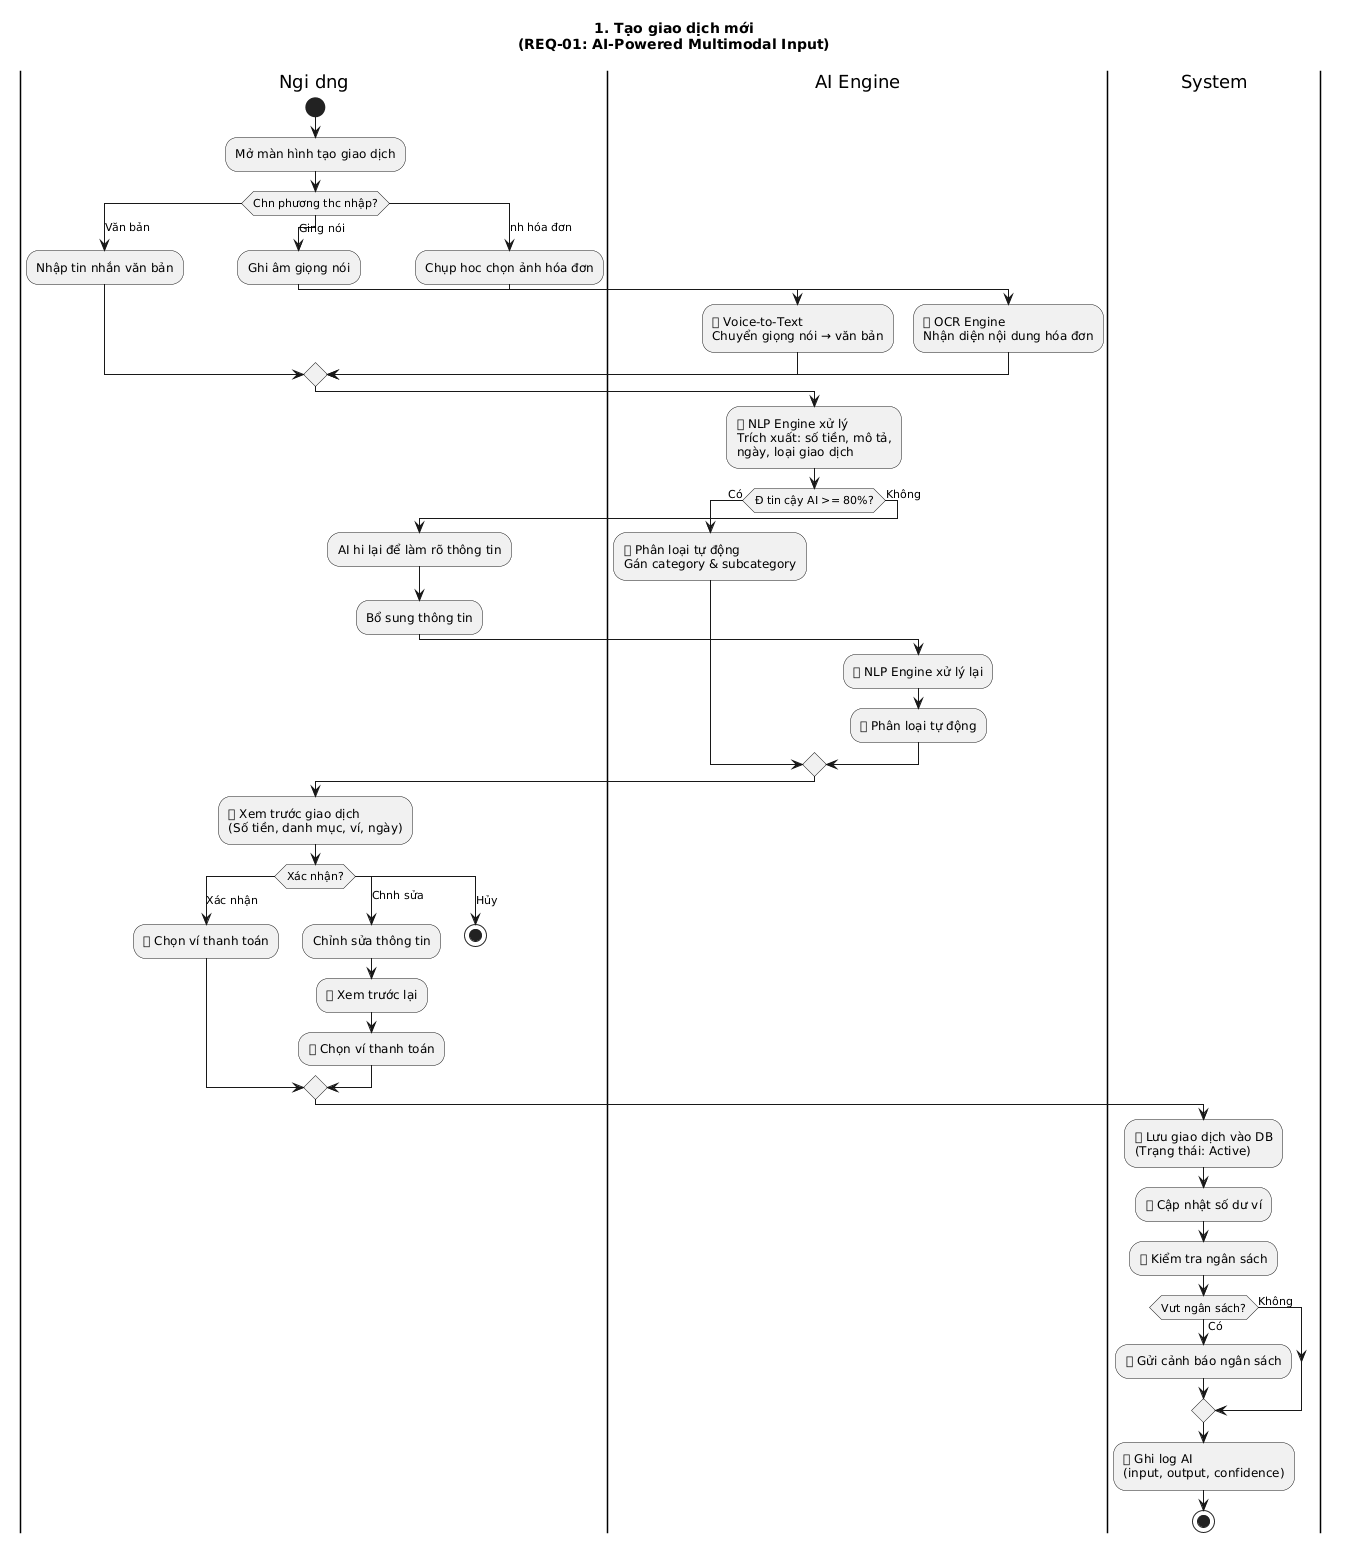
\includegraphics[width=0.85\textwidth]{images/activity-tạo-giao-dịch-mớinreq-01-ai-powered-multimodal-input.png}
    \caption{Sơ đồ hoạt động: Tạo giao dịch mới (REQ-01)}
    \label{fig:act_create_trans}
\end{figure}

\begin{figure}[htbp]
    \centering
    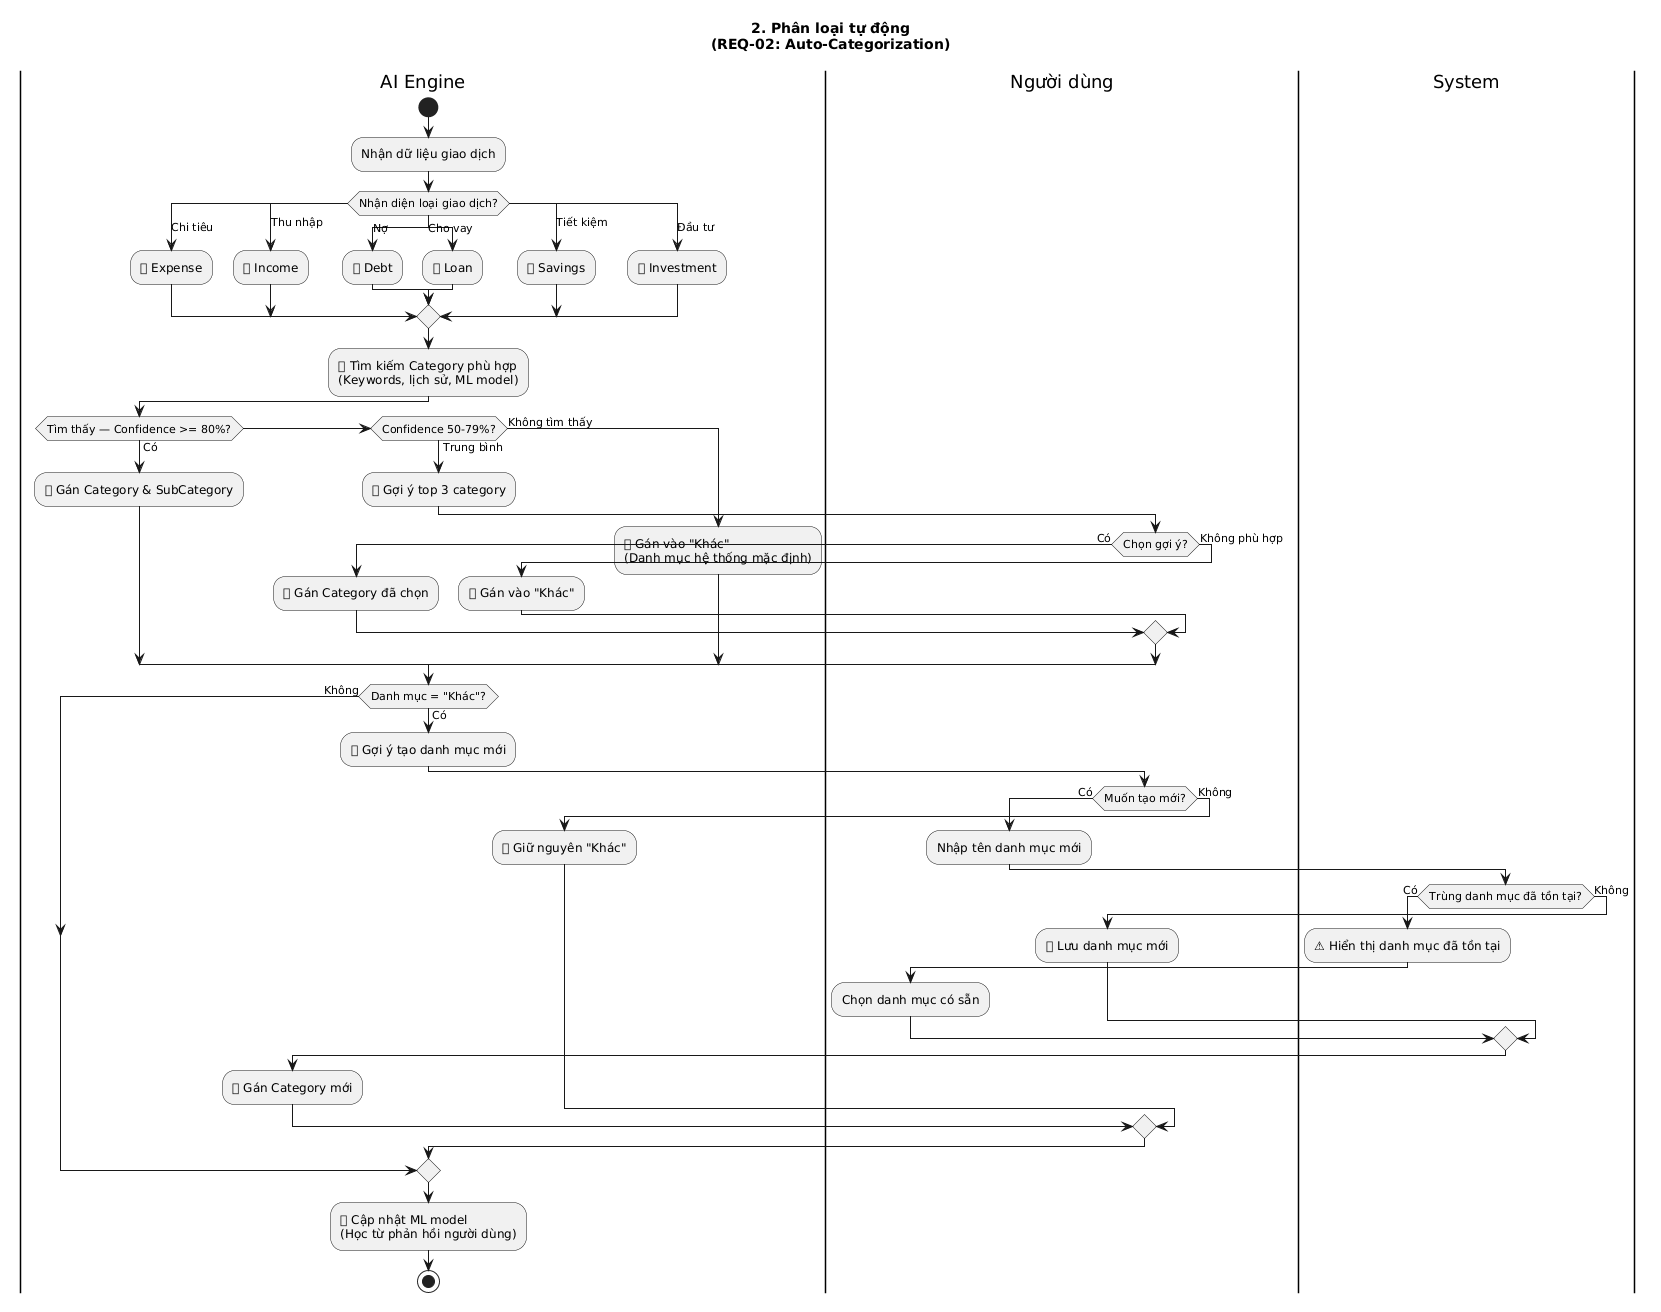
\includegraphics[width=0.85\textwidth]{images/activity-phân-loại-tự-độngnreq-02-auto-categorization.png}
    \caption{Sơ đồ hoạt động: Phân loại tự động (REQ-02)}
    \label{fig:act_auto_cat}
\end{figure}

\begin{figure}[htbp]
    \centering
    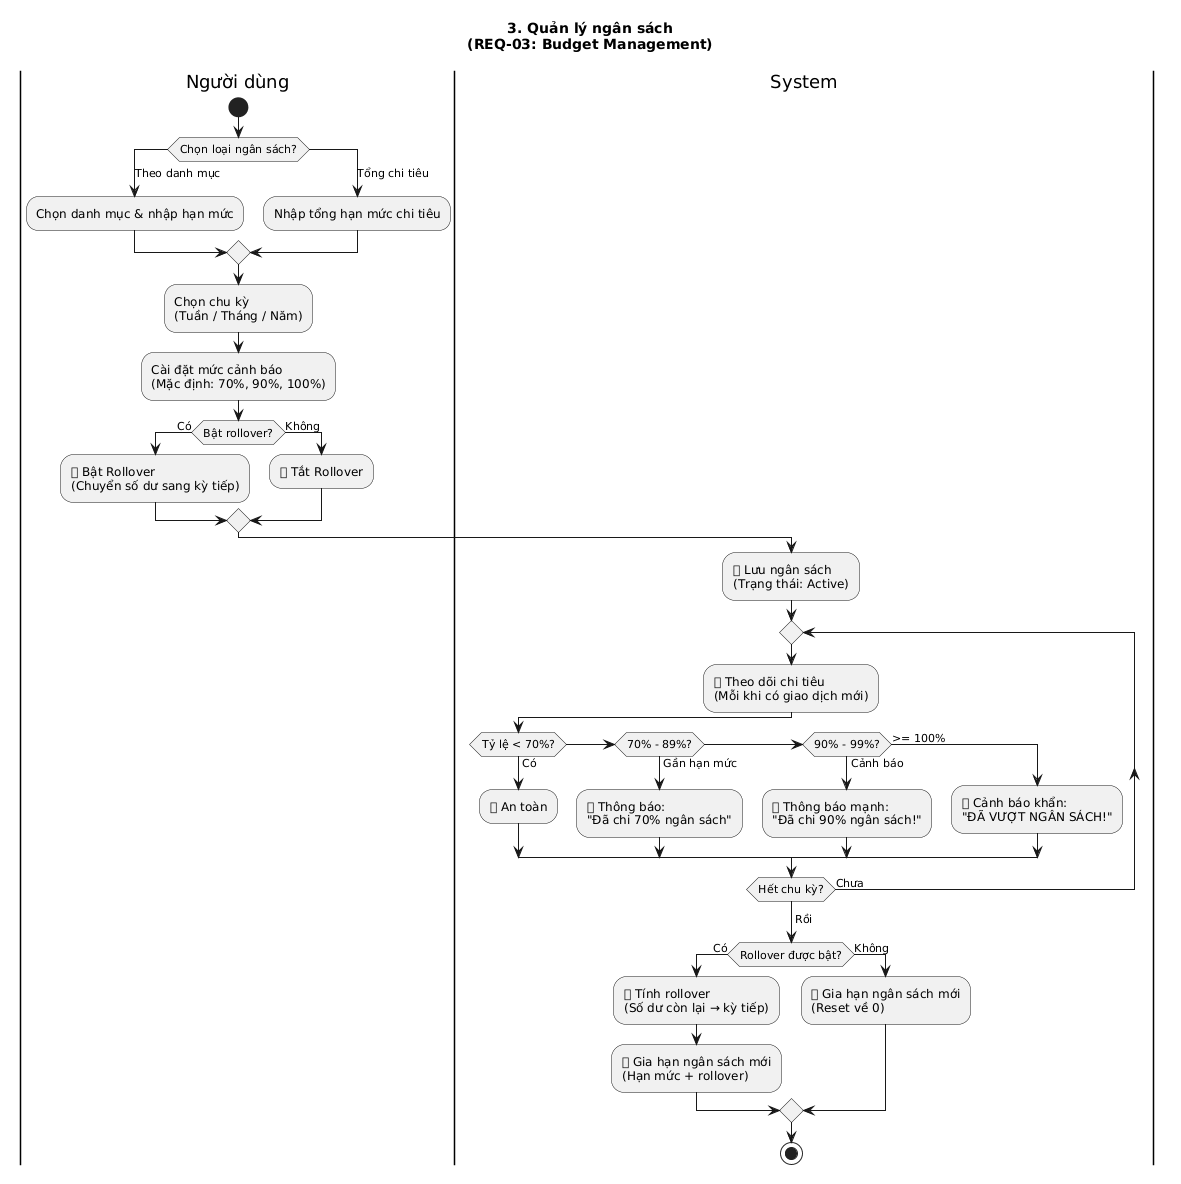
\includegraphics[width=0.85\textwidth]{images/activity-quản-lý-ngân-sáchnreq-03-budget-management.png}
    \caption{Sơ đồ hoạt động: Quản lý ngân sách (REQ-03)}
    \label{fig:act_budget_mgmt}
\end{figure}

\begin{figure}[htbp]
    \centering
    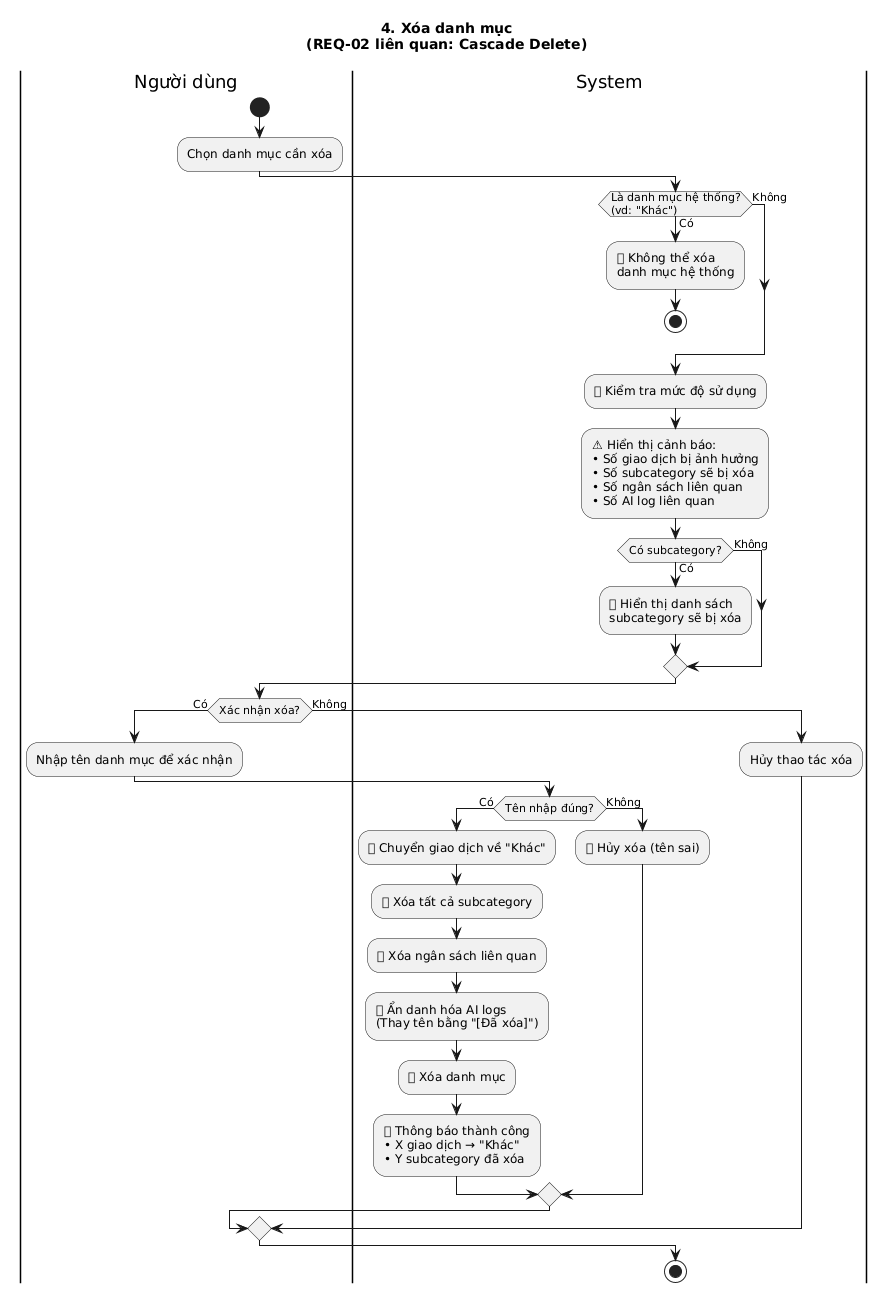
\includegraphics[width=0.85\textwidth]{images/activity-xóa-danh-mụcnreq-02-liên-quan-cascade-delete.png}
    \caption{Sơ đồ hoạt động: Xóa danh mục (REQ-02)}
    \label{fig:act_delete_cat}
\end{figure}

\begin{figure}[htbp]
    \centering
    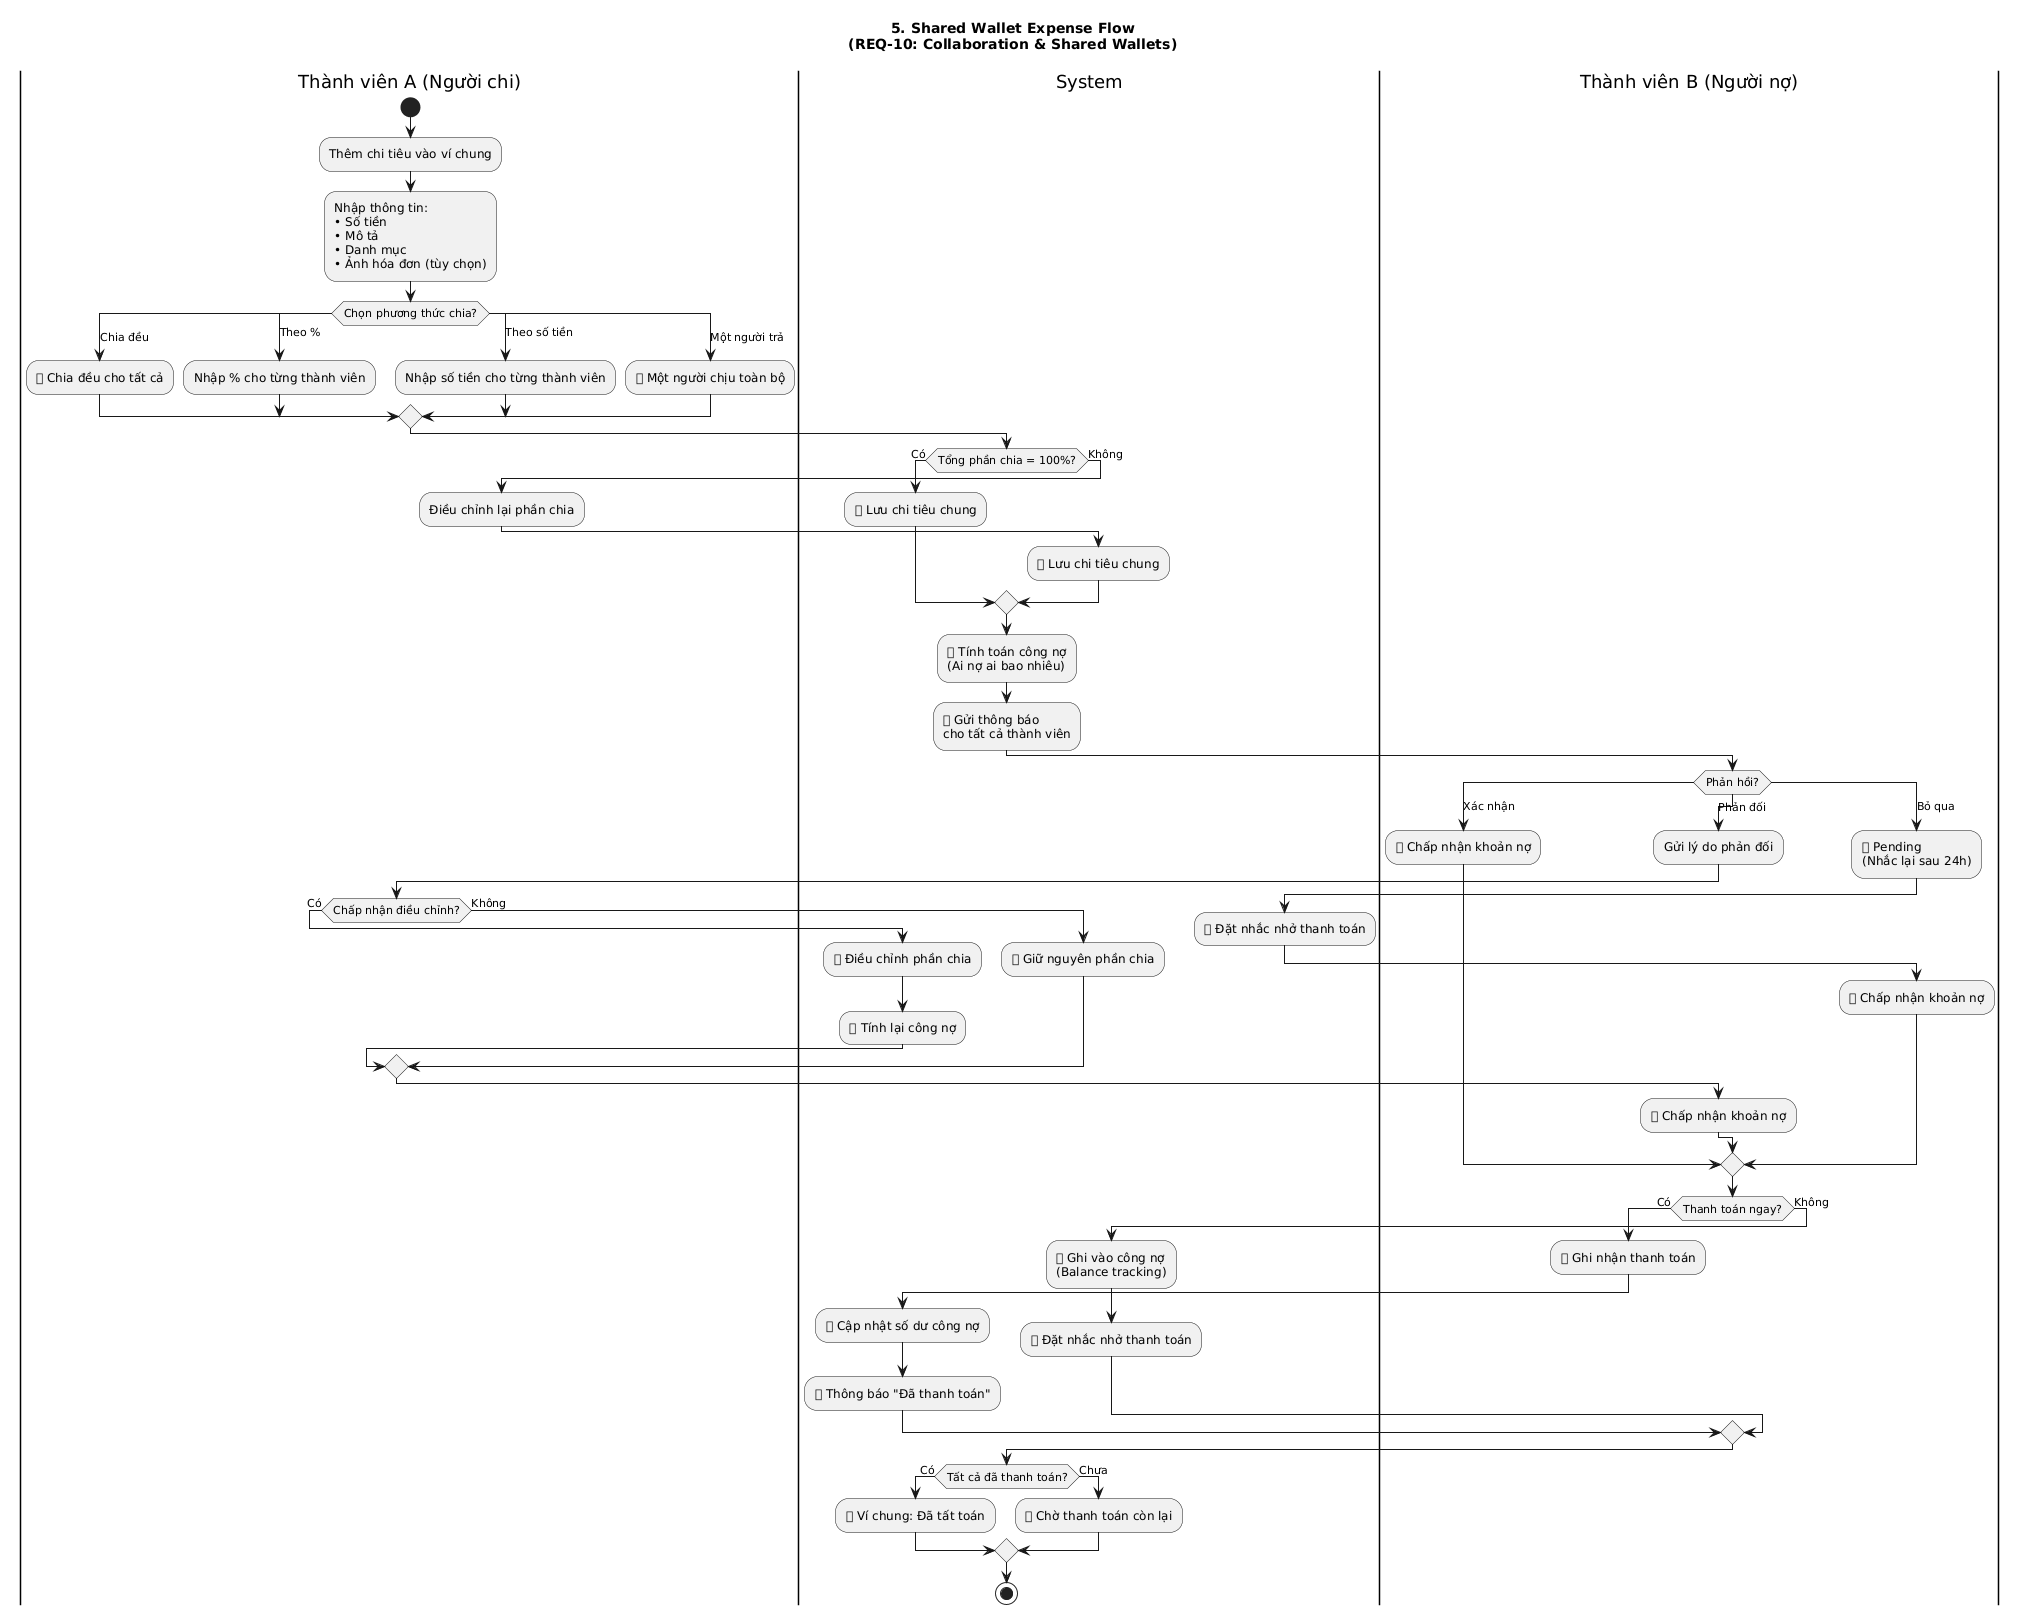
\includegraphics[width=0.85\textwidth]{images/activity-shared-wallet-expense-flownreq-10-collaboration-shared-wallets.png}
    \caption{Sơ đồ hoạt động: Quy trình chi tiêu ví chung (REQ-10)}
    \label{fig:act_shared_wallet}
\end{figure}

[TODO --- Giải thích quy trình xử lý chi tiết]

\subsubsection{Thiết kế giao diện người dùng (UI Design)}
[TODO --- Trình bày wireframe/mockup cho các màn hình chính:
\begin{enumerate}
    \item Màn hình Chat (giao diện chính)
    \item Màn hình Dashboard/Tổng quan
    \item Màn hình Báo cáo/Biểu đồ
    \item Màn hình Quản lý Ngân sách
    \item Màn hình Quản lý Ví/Tài khoản
    \item Màn hình Cài đặt
\end{enumerate}
]

\subsubsection{Mô tả thuật toán và kỹ thuật quan trọng}
[TODO --- Giải thích chi tiết:
\begin{enumerate}
    \item Luồng xử lý NLP: từ input text $\rightarrow$ intent classification $\rightarrow$ entity extraction $\rightarrow$ transaction creation
    \item Luồng xử lý OCR: từ image $\rightarrow$ preprocessing $\rightarrow$ text detection $\rightarrow$ structured data extraction
    \item Thuật toán phân loại danh mục: prompt engineering cho LLM, feedback loop
    \item Thuật toán phát hiện bất thường chi tiêu
    \item Cơ chế cảnh báo ngân sách proactive
\end{enumerate}
]

\section{Kiểm thử (Testing)}
\label{sec:testing}

\subsection{Kế hoạch kiểm thử (Test Plan)}
\label{subsec:test_plan}

[TODO --- Trình bày chiến lược kiểm thử bao gồm:]

\subsubsection{Các loại kiểm thử}

\begin{table}[htbp]
\centering
\begin{tabularx}{\textwidth}{|l|X|l|}
\hline
\textbf{Loại kiểm thử} & \textbf{Mô tả} & \textbf{Công cụ} \\ \hline
Unit Testing & Kiểm thử từng hàm/module riêng lẻ & [TODO] \\ \hline
Integration Testing & Kiểm thử tích hợp giữa các service & [TODO] \\ \hline
System Testing & Kiểm thử toàn hệ thống end-to-end & [TODO] \\ \hline
User Acceptance Testing & Kiểm thử chấp nhận với người dùng thực & [TODO] \\ \hline
\end{tabularx}
\caption{Kế hoạch kiểm thử}
\label{tab:test_plan}
\end{table}

\subsubsection{Các test case chính}

[TODO --- Liệt kê test case cho các luồng quan trọng:]

\begin{table}[htbp]
\centering
\begin{tabularx}{\textwidth}{|l|p{3.5cm}|X|p{2cm}|p{2cm}|p{1.5cm}|}
\hline
\textbf{Mã TC} & \textbf{Mô tả} & \textbf{Đầu vào} & \textbf{Kết quả mong đợi} & \textbf{Kết quả thực tế} & \textbf{Trạng thái} \\ \hline
TC-01 & Nhập giao dịch bằng văn bản tiếng Việt & "trà sữa 50k" & Tạo giao dịch: tên="trà sữa", số tiền=50.000đ, danh mục="Ăn uống" & [TODO] & [TODO] \\ \hline
TC-02 & Nhập giao dịch bằng hình ảnh hóa đơn & Ảnh hóa đơn siêu thị & Trích xuất danh sách sản phẩm và tổng tiền & [TODO] & [TODO] \\ \hline
TC-03 & Cảnh báo ngân sách 70\% & Chi tiêu vượt 70\% hạn mức & Hệ thống gửi cảnh báo trong chat & [TODO] & [TODO] \\ \hline
TC-04 & Phân loại tự động & "grab đi làm 30k" & Giao dịch phân loại vào "Di chuyển" & [TODO] & [TODO] \\ \hline
\end{tabularx}
\caption{Các test case chính}
\label{tab:test_cases}
\end{table}

[TODO --- Bổ sung thêm test case]

\subsection{Kết quả và phân tích (Results \& Analysis)}
\label{subsec:test_results}

[TODO --- Trình bày kết quả kiểm thử và sử dụng bảng, biểu đồ để minh họa:
\begin{itemize}
    \item Tỷ lệ pass/fail của test case
    \item Độ chính xác phân loại danh mục
    \item Thời gian phản hồi trung bình
    \item Kết quả UAT
\end{itemize}
]
